
% Default to the notebook output style

    


% Inherit from the specified cell style.




    
\documentclass[11pt]{article}

    
    
    \usepackage[T1]{fontenc}
    % Nicer default font (+ math font) than Computer Modern for most use cases
    \usepackage{mathpazo}

    % Basic figure setup, for now with no caption control since it's done
    % automatically by Pandoc (which extracts ![](path) syntax from Markdown).
    \usepackage{graphicx}
    % We will generate all images so they have a width \maxwidth. This means
    % that they will get their normal width if they fit onto the page, but
    % are scaled down if they would overflow the margins.
    \makeatletter
    \def\maxwidth{\ifdim\Gin@nat@width>\linewidth\linewidth
    \else\Gin@nat@width\fi}
    \makeatother
    \let\Oldincludegraphics\includegraphics
    % Set max figure width to be 80% of text width, for now hardcoded.
    \renewcommand{\includegraphics}[1]{\Oldincludegraphics[width=.8\maxwidth]{#1}}
    % Ensure that by default, figures have no caption (until we provide a
    % proper Figure object with a Caption API and a way to capture that
    % in the conversion process - todo).
    \usepackage{caption}
    \DeclareCaptionLabelFormat{nolabel}{}
    \captionsetup{labelformat=nolabel}

    \usepackage{adjustbox} % Used to constrain images to a maximum size 
    \usepackage{xcolor} % Allow colors to be defined
    \usepackage{enumerate} % Needed for markdown enumerations to work
    \usepackage{geometry} % Used to adjust the document margins
    \usepackage{amsmath} % Equations
    \usepackage{amssymb} % Equations
    \usepackage{textcomp} % defines textquotesingle
    % Hack from http://tex.stackexchange.com/a/47451/13684:
    \AtBeginDocument{%
        \def\PYZsq{\textquotesingle}% Upright quotes in Pygmentized code
    }
    \usepackage{upquote} % Upright quotes for verbatim code
    \usepackage{eurosym} % defines \euro
    \usepackage[mathletters]{ucs} % Extended unicode (utf-8) support
    \usepackage[utf8x]{inputenc} % Allow utf-8 characters in the tex document
    \usepackage{fancyvrb} % verbatim replacement that allows latex
    \usepackage{grffile} % extends the file name processing of package graphics 
                         % to support a larger range 
    % The hyperref package gives us a pdf with properly built
    % internal navigation ('pdf bookmarks' for the table of contents,
    % internal cross-reference links, web links for URLs, etc.)
    \usepackage{hyperref}
    \usepackage{longtable} % longtable support required by pandoc >1.10
    \usepackage{booktabs}  % table support for pandoc > 1.12.2
    \usepackage[inline]{enumitem} % IRkernel/repr support (it uses the enumerate* environment)
    \usepackage[normalem]{ulem} % ulem is needed to support strikethroughs (\sout)
                                % normalem makes italics be italics, not underlines
    

    
    
    % Colors for the hyperref package
    \definecolor{urlcolor}{rgb}{0,.145,.698}
    \definecolor{linkcolor}{rgb}{.71,0.21,0.01}
    \definecolor{citecolor}{rgb}{.12,.54,.11}

    % ANSI colors
    \definecolor{ansi-black}{HTML}{3E424D}
    \definecolor{ansi-black-intense}{HTML}{282C36}
    \definecolor{ansi-red}{HTML}{E75C58}
    \definecolor{ansi-red-intense}{HTML}{B22B31}
    \definecolor{ansi-green}{HTML}{00A250}
    \definecolor{ansi-green-intense}{HTML}{007427}
    \definecolor{ansi-yellow}{HTML}{DDB62B}
    \definecolor{ansi-yellow-intense}{HTML}{B27D12}
    \definecolor{ansi-blue}{HTML}{208FFB}
    \definecolor{ansi-blue-intense}{HTML}{0065CA}
    \definecolor{ansi-magenta}{HTML}{D160C4}
    \definecolor{ansi-magenta-intense}{HTML}{A03196}
    \definecolor{ansi-cyan}{HTML}{60C6C8}
    \definecolor{ansi-cyan-intense}{HTML}{258F8F}
    \definecolor{ansi-white}{HTML}{C5C1B4}
    \definecolor{ansi-white-intense}{HTML}{A1A6B2}

    % commands and environments needed by pandoc snippets
    % extracted from the output of `pandoc -s`
    \providecommand{\tightlist}{%
      \setlength{\itemsep}{0pt}\setlength{\parskip}{0pt}}
    \DefineVerbatimEnvironment{Highlighting}{Verbatim}{commandchars=\\\{\}}
    % Add ',fontsize=\small' for more characters per line
    \newenvironment{Shaded}{}{}
    \newcommand{\KeywordTok}[1]{\textcolor[rgb]{0.00,0.44,0.13}{\textbf{{#1}}}}
    \newcommand{\DataTypeTok}[1]{\textcolor[rgb]{0.56,0.13,0.00}{{#1}}}
    \newcommand{\DecValTok}[1]{\textcolor[rgb]{0.25,0.63,0.44}{{#1}}}
    \newcommand{\BaseNTok}[1]{\textcolor[rgb]{0.25,0.63,0.44}{{#1}}}
    \newcommand{\FloatTok}[1]{\textcolor[rgb]{0.25,0.63,0.44}{{#1}}}
    \newcommand{\CharTok}[1]{\textcolor[rgb]{0.25,0.44,0.63}{{#1}}}
    \newcommand{\StringTok}[1]{\textcolor[rgb]{0.25,0.44,0.63}{{#1}}}
    \newcommand{\CommentTok}[1]{\textcolor[rgb]{0.38,0.63,0.69}{\textit{{#1}}}}
    \newcommand{\OtherTok}[1]{\textcolor[rgb]{0.00,0.44,0.13}{{#1}}}
    \newcommand{\AlertTok}[1]{\textcolor[rgb]{1.00,0.00,0.00}{\textbf{{#1}}}}
    \newcommand{\FunctionTok}[1]{\textcolor[rgb]{0.02,0.16,0.49}{{#1}}}
    \newcommand{\RegionMarkerTok}[1]{{#1}}
    \newcommand{\ErrorTok}[1]{\textcolor[rgb]{1.00,0.00,0.00}{\textbf{{#1}}}}
    \newcommand{\NormalTok}[1]{{#1}}
    
    % Additional commands for more recent versions of Pandoc
    \newcommand{\ConstantTok}[1]{\textcolor[rgb]{0.53,0.00,0.00}{{#1}}}
    \newcommand{\SpecialCharTok}[1]{\textcolor[rgb]{0.25,0.44,0.63}{{#1}}}
    \newcommand{\VerbatimStringTok}[1]{\textcolor[rgb]{0.25,0.44,0.63}{{#1}}}
    \newcommand{\SpecialStringTok}[1]{\textcolor[rgb]{0.73,0.40,0.53}{{#1}}}
    \newcommand{\ImportTok}[1]{{#1}}
    \newcommand{\DocumentationTok}[1]{\textcolor[rgb]{0.73,0.13,0.13}{\textit{{#1}}}}
    \newcommand{\AnnotationTok}[1]{\textcolor[rgb]{0.38,0.63,0.69}{\textbf{\textit{{#1}}}}}
    \newcommand{\CommentVarTok}[1]{\textcolor[rgb]{0.38,0.63,0.69}{\textbf{\textit{{#1}}}}}
    \newcommand{\VariableTok}[1]{\textcolor[rgb]{0.10,0.09,0.49}{{#1}}}
    \newcommand{\ControlFlowTok}[1]{\textcolor[rgb]{0.00,0.44,0.13}{\textbf{{#1}}}}
    \newcommand{\OperatorTok}[1]{\textcolor[rgb]{0.40,0.40,0.40}{{#1}}}
    \newcommand{\BuiltInTok}[1]{{#1}}
    \newcommand{\ExtensionTok}[1]{{#1}}
    \newcommand{\PreprocessorTok}[1]{\textcolor[rgb]{0.74,0.48,0.00}{{#1}}}
    \newcommand{\AttributeTok}[1]{\textcolor[rgb]{0.49,0.56,0.16}{{#1}}}
    \newcommand{\InformationTok}[1]{\textcolor[rgb]{0.38,0.63,0.69}{\textbf{\textit{{#1}}}}}
    \newcommand{\WarningTok}[1]{\textcolor[rgb]{0.38,0.63,0.69}{\textbf{\textit{{#1}}}}}
    
    
    % Define a nice break command that doesn't care if a line doesn't already
    % exist.
    \def\br{\hspace*{\fill} \\* }
    % Math Jax compatability definitions
    \def\gt{>}
    \def\lt{<}
    % Document parameters
    \title{final-project-cellon}
    
    
    

    % Pygments definitions
    
\makeatletter
\def\PY@reset{\let\PY@it=\relax \let\PY@bf=\relax%
    \let\PY@ul=\relax \let\PY@tc=\relax%
    \let\PY@bc=\relax \let\PY@ff=\relax}
\def\PY@tok#1{\csname PY@tok@#1\endcsname}
\def\PY@toks#1+{\ifx\relax#1\empty\else%
    \PY@tok{#1}\expandafter\PY@toks\fi}
\def\PY@do#1{\PY@bc{\PY@tc{\PY@ul{%
    \PY@it{\PY@bf{\PY@ff{#1}}}}}}}
\def\PY#1#2{\PY@reset\PY@toks#1+\relax+\PY@do{#2}}

\expandafter\def\csname PY@tok@w\endcsname{\def\PY@tc##1{\textcolor[rgb]{0.73,0.73,0.73}{##1}}}
\expandafter\def\csname PY@tok@c\endcsname{\let\PY@it=\textit\def\PY@tc##1{\textcolor[rgb]{0.25,0.50,0.50}{##1}}}
\expandafter\def\csname PY@tok@cp\endcsname{\def\PY@tc##1{\textcolor[rgb]{0.74,0.48,0.00}{##1}}}
\expandafter\def\csname PY@tok@k\endcsname{\let\PY@bf=\textbf\def\PY@tc##1{\textcolor[rgb]{0.00,0.50,0.00}{##1}}}
\expandafter\def\csname PY@tok@kp\endcsname{\def\PY@tc##1{\textcolor[rgb]{0.00,0.50,0.00}{##1}}}
\expandafter\def\csname PY@tok@kt\endcsname{\def\PY@tc##1{\textcolor[rgb]{0.69,0.00,0.25}{##1}}}
\expandafter\def\csname PY@tok@o\endcsname{\def\PY@tc##1{\textcolor[rgb]{0.40,0.40,0.40}{##1}}}
\expandafter\def\csname PY@tok@ow\endcsname{\let\PY@bf=\textbf\def\PY@tc##1{\textcolor[rgb]{0.67,0.13,1.00}{##1}}}
\expandafter\def\csname PY@tok@nb\endcsname{\def\PY@tc##1{\textcolor[rgb]{0.00,0.50,0.00}{##1}}}
\expandafter\def\csname PY@tok@nf\endcsname{\def\PY@tc##1{\textcolor[rgb]{0.00,0.00,1.00}{##1}}}
\expandafter\def\csname PY@tok@nc\endcsname{\let\PY@bf=\textbf\def\PY@tc##1{\textcolor[rgb]{0.00,0.00,1.00}{##1}}}
\expandafter\def\csname PY@tok@nn\endcsname{\let\PY@bf=\textbf\def\PY@tc##1{\textcolor[rgb]{0.00,0.00,1.00}{##1}}}
\expandafter\def\csname PY@tok@ne\endcsname{\let\PY@bf=\textbf\def\PY@tc##1{\textcolor[rgb]{0.82,0.25,0.23}{##1}}}
\expandafter\def\csname PY@tok@nv\endcsname{\def\PY@tc##1{\textcolor[rgb]{0.10,0.09,0.49}{##1}}}
\expandafter\def\csname PY@tok@no\endcsname{\def\PY@tc##1{\textcolor[rgb]{0.53,0.00,0.00}{##1}}}
\expandafter\def\csname PY@tok@nl\endcsname{\def\PY@tc##1{\textcolor[rgb]{0.63,0.63,0.00}{##1}}}
\expandafter\def\csname PY@tok@ni\endcsname{\let\PY@bf=\textbf\def\PY@tc##1{\textcolor[rgb]{0.60,0.60,0.60}{##1}}}
\expandafter\def\csname PY@tok@na\endcsname{\def\PY@tc##1{\textcolor[rgb]{0.49,0.56,0.16}{##1}}}
\expandafter\def\csname PY@tok@nt\endcsname{\let\PY@bf=\textbf\def\PY@tc##1{\textcolor[rgb]{0.00,0.50,0.00}{##1}}}
\expandafter\def\csname PY@tok@nd\endcsname{\def\PY@tc##1{\textcolor[rgb]{0.67,0.13,1.00}{##1}}}
\expandafter\def\csname PY@tok@s\endcsname{\def\PY@tc##1{\textcolor[rgb]{0.73,0.13,0.13}{##1}}}
\expandafter\def\csname PY@tok@sd\endcsname{\let\PY@it=\textit\def\PY@tc##1{\textcolor[rgb]{0.73,0.13,0.13}{##1}}}
\expandafter\def\csname PY@tok@si\endcsname{\let\PY@bf=\textbf\def\PY@tc##1{\textcolor[rgb]{0.73,0.40,0.53}{##1}}}
\expandafter\def\csname PY@tok@se\endcsname{\let\PY@bf=\textbf\def\PY@tc##1{\textcolor[rgb]{0.73,0.40,0.13}{##1}}}
\expandafter\def\csname PY@tok@sr\endcsname{\def\PY@tc##1{\textcolor[rgb]{0.73,0.40,0.53}{##1}}}
\expandafter\def\csname PY@tok@ss\endcsname{\def\PY@tc##1{\textcolor[rgb]{0.10,0.09,0.49}{##1}}}
\expandafter\def\csname PY@tok@sx\endcsname{\def\PY@tc##1{\textcolor[rgb]{0.00,0.50,0.00}{##1}}}
\expandafter\def\csname PY@tok@m\endcsname{\def\PY@tc##1{\textcolor[rgb]{0.40,0.40,0.40}{##1}}}
\expandafter\def\csname PY@tok@gh\endcsname{\let\PY@bf=\textbf\def\PY@tc##1{\textcolor[rgb]{0.00,0.00,0.50}{##1}}}
\expandafter\def\csname PY@tok@gu\endcsname{\let\PY@bf=\textbf\def\PY@tc##1{\textcolor[rgb]{0.50,0.00,0.50}{##1}}}
\expandafter\def\csname PY@tok@gd\endcsname{\def\PY@tc##1{\textcolor[rgb]{0.63,0.00,0.00}{##1}}}
\expandafter\def\csname PY@tok@gi\endcsname{\def\PY@tc##1{\textcolor[rgb]{0.00,0.63,0.00}{##1}}}
\expandafter\def\csname PY@tok@gr\endcsname{\def\PY@tc##1{\textcolor[rgb]{1.00,0.00,0.00}{##1}}}
\expandafter\def\csname PY@tok@ge\endcsname{\let\PY@it=\textit}
\expandafter\def\csname PY@tok@gs\endcsname{\let\PY@bf=\textbf}
\expandafter\def\csname PY@tok@gp\endcsname{\let\PY@bf=\textbf\def\PY@tc##1{\textcolor[rgb]{0.00,0.00,0.50}{##1}}}
\expandafter\def\csname PY@tok@go\endcsname{\def\PY@tc##1{\textcolor[rgb]{0.53,0.53,0.53}{##1}}}
\expandafter\def\csname PY@tok@gt\endcsname{\def\PY@tc##1{\textcolor[rgb]{0.00,0.27,0.87}{##1}}}
\expandafter\def\csname PY@tok@err\endcsname{\def\PY@bc##1{\setlength{\fboxsep}{0pt}\fcolorbox[rgb]{1.00,0.00,0.00}{1,1,1}{\strut ##1}}}
\expandafter\def\csname PY@tok@kc\endcsname{\let\PY@bf=\textbf\def\PY@tc##1{\textcolor[rgb]{0.00,0.50,0.00}{##1}}}
\expandafter\def\csname PY@tok@kd\endcsname{\let\PY@bf=\textbf\def\PY@tc##1{\textcolor[rgb]{0.00,0.50,0.00}{##1}}}
\expandafter\def\csname PY@tok@kn\endcsname{\let\PY@bf=\textbf\def\PY@tc##1{\textcolor[rgb]{0.00,0.50,0.00}{##1}}}
\expandafter\def\csname PY@tok@kr\endcsname{\let\PY@bf=\textbf\def\PY@tc##1{\textcolor[rgb]{0.00,0.50,0.00}{##1}}}
\expandafter\def\csname PY@tok@bp\endcsname{\def\PY@tc##1{\textcolor[rgb]{0.00,0.50,0.00}{##1}}}
\expandafter\def\csname PY@tok@fm\endcsname{\def\PY@tc##1{\textcolor[rgb]{0.00,0.00,1.00}{##1}}}
\expandafter\def\csname PY@tok@vc\endcsname{\def\PY@tc##1{\textcolor[rgb]{0.10,0.09,0.49}{##1}}}
\expandafter\def\csname PY@tok@vg\endcsname{\def\PY@tc##1{\textcolor[rgb]{0.10,0.09,0.49}{##1}}}
\expandafter\def\csname PY@tok@vi\endcsname{\def\PY@tc##1{\textcolor[rgb]{0.10,0.09,0.49}{##1}}}
\expandafter\def\csname PY@tok@vm\endcsname{\def\PY@tc##1{\textcolor[rgb]{0.10,0.09,0.49}{##1}}}
\expandafter\def\csname PY@tok@sa\endcsname{\def\PY@tc##1{\textcolor[rgb]{0.73,0.13,0.13}{##1}}}
\expandafter\def\csname PY@tok@sb\endcsname{\def\PY@tc##1{\textcolor[rgb]{0.73,0.13,0.13}{##1}}}
\expandafter\def\csname PY@tok@sc\endcsname{\def\PY@tc##1{\textcolor[rgb]{0.73,0.13,0.13}{##1}}}
\expandafter\def\csname PY@tok@dl\endcsname{\def\PY@tc##1{\textcolor[rgb]{0.73,0.13,0.13}{##1}}}
\expandafter\def\csname PY@tok@s2\endcsname{\def\PY@tc##1{\textcolor[rgb]{0.73,0.13,0.13}{##1}}}
\expandafter\def\csname PY@tok@sh\endcsname{\def\PY@tc##1{\textcolor[rgb]{0.73,0.13,0.13}{##1}}}
\expandafter\def\csname PY@tok@s1\endcsname{\def\PY@tc##1{\textcolor[rgb]{0.73,0.13,0.13}{##1}}}
\expandafter\def\csname PY@tok@mb\endcsname{\def\PY@tc##1{\textcolor[rgb]{0.40,0.40,0.40}{##1}}}
\expandafter\def\csname PY@tok@mf\endcsname{\def\PY@tc##1{\textcolor[rgb]{0.40,0.40,0.40}{##1}}}
\expandafter\def\csname PY@tok@mh\endcsname{\def\PY@tc##1{\textcolor[rgb]{0.40,0.40,0.40}{##1}}}
\expandafter\def\csname PY@tok@mi\endcsname{\def\PY@tc##1{\textcolor[rgb]{0.40,0.40,0.40}{##1}}}
\expandafter\def\csname PY@tok@il\endcsname{\def\PY@tc##1{\textcolor[rgb]{0.40,0.40,0.40}{##1}}}
\expandafter\def\csname PY@tok@mo\endcsname{\def\PY@tc##1{\textcolor[rgb]{0.40,0.40,0.40}{##1}}}
\expandafter\def\csname PY@tok@ch\endcsname{\let\PY@it=\textit\def\PY@tc##1{\textcolor[rgb]{0.25,0.50,0.50}{##1}}}
\expandafter\def\csname PY@tok@cm\endcsname{\let\PY@it=\textit\def\PY@tc##1{\textcolor[rgb]{0.25,0.50,0.50}{##1}}}
\expandafter\def\csname PY@tok@cpf\endcsname{\let\PY@it=\textit\def\PY@tc##1{\textcolor[rgb]{0.25,0.50,0.50}{##1}}}
\expandafter\def\csname PY@tok@c1\endcsname{\let\PY@it=\textit\def\PY@tc##1{\textcolor[rgb]{0.25,0.50,0.50}{##1}}}
\expandafter\def\csname PY@tok@cs\endcsname{\let\PY@it=\textit\def\PY@tc##1{\textcolor[rgb]{0.25,0.50,0.50}{##1}}}

\def\PYZbs{\char`\\}
\def\PYZus{\char`\_}
\def\PYZob{\char`\{}
\def\PYZcb{\char`\}}
\def\PYZca{\char`\^}
\def\PYZam{\char`\&}
\def\PYZlt{\char`\<}
\def\PYZgt{\char`\>}
\def\PYZsh{\char`\#}
\def\PYZpc{\char`\%}
\def\PYZdl{\char`\$}
\def\PYZhy{\char`\-}
\def\PYZsq{\char`\'}
\def\PYZdq{\char`\"}
\def\PYZti{\char`\~}
% for compatibility with earlier versions
\def\PYZat{@}
\def\PYZlb{[}
\def\PYZrb{]}
\makeatother


    % Exact colors from NB
    \definecolor{incolor}{rgb}{0.0, 0.0, 0.5}
    \definecolor{outcolor}{rgb}{0.545, 0.0, 0.0}



    
    % Prevent overflowing lines due to hard-to-break entities
    \sloppy 
    % Setup hyperref package
    \hypersetup{
      breaklinks=true,  % so long urls are correctly broken across lines
      colorlinks=true,
      urlcolor=urlcolor,
      linkcolor=linkcolor,
      citecolor=citecolor,
      }
    % Slightly bigger margins than the latex defaults
    
    \geometry{verbose,tmargin=1in,bmargin=1in,lmargin=1in,rmargin=1in}
    
    

    \begin{document}
    
    
    \maketitle
    
    

    
    \hypertarget{emerging-models-of-computation-final-project}{%
\section{Emerging Models of Computation Final
Project}\label{emerging-models-of-computation-final-project}}

Adam Cellon

    \begin{Verbatim}[commandchars=\\\{\}]
{\color{incolor}In [{\color{incolor}1}]:} \PY{k+kn}{from} \PY{n+nn}{brian2} \PY{k}{import} \PY{o}{*}
        
        \PY{o}{\PYZpc{}}\PY{k}{matplotlib} inline
\end{Verbatim}


    First, let's describe the dynamics of the saturating synapse model. We
choose this model because it is simpler to adapt to the Brian2 simulator
than the nonlinear dendritic model, but is still able to produce the
arbitrary encoding of continuous signals.

\[
\begin{eqnarray}
s_n(t)       &=& \sum_{t_n} \delta ( t - t_n) \\
\dot{r_n}(t) &=& -\lambda_s r_n(t) + s_n(t) \\
\dot{V_n}(t) &=& -\lambda_V V_n(t) + \sum_{m=1}^T A_{nm} \tanh{(\gamma r_m(t))} + V_r \lambda_s r_n(t) - \theta s_n(t) + I_{e,n}(t) \\
\end{eqnarray}
\]

Next, let's describe each of the various parameters and variables
necessary to implement the model:

\begin{itemize}
\tightlist
\item
  Incoming spiketrain, \(s(t)\)

  \begin{itemize}
  \tightlist
  \item
    Just a train of delta impulses - no parameters needed.
  \item
    Simply increment on-spike with Brian2
  \end{itemize}
\item
  Normalized synaptic current, \(r(t)\)

  \begin{itemize}
  \tightlist
  \item
    \(\lambda_s = \tau_s^{-1}\) : time constant of synaptic decay
    (consistent for all synapses in this model)
  \end{itemize}
\item
  Membrane potential, \(V(t)\)

  \begin{itemize}
  \tightlist
  \item
    \(\lambda_V = \tau_m^{-1}\) : membrane time constant for neuron
  \item
    \(A_{nm}\) : maximum synapse strength from neuron \texttt{m} to
    neuron \texttt{n}
  \item
    \(\gamma\) : ``fraction of synaptic resources consumed'' by the
    synapse
  \item
    \(V_r\) : resting voltage (temporally integrated size of
    afterdepolarization recovery current)
  \item
    \(\theta\) : threshold voltage (compared to reset voltage)
  \item
    \(I_{e,n}\) : external input current
  \end{itemize}
\end{itemize}

Now, let's set some of those parameters. I began with those defined in
the paper and supplemental materials, but changed various parameters to
better find a suitable output.

    \begin{Verbatim}[commandchars=\\\{\}]
{\color{incolor}In [{\color{incolor}2}]:} \PY{c+c1}{\PYZsh{} Set model parameters}
        
        \PY{n}{lambda\PYZus{}s} \PY{o}{=} \PY{l+m+mi}{1} \PY{o}{*} \PY{n}{Hz}
        \PY{n}{lambda\PYZus{}v} \PY{o}{=} \PY{l+m+mf}{0.1} \PY{o}{*} \PY{n}{Hz}
        
        \PY{n}{theta} \PY{o}{=} \PY{l+m+mf}{0.1} \PY{c+c1}{\PYZsh{} increasing theta decreases spikerate}
        \PY{n}{gamma} \PY{o}{=} \PY{l+m+mf}{0.05}
        \PY{n}{V\PYZus{}r} \PY{o}{=} \PY{l+m+mf}{0.9} \PY{o}{*} \PY{n}{theta}
        
        \PY{n}{N} \PY{o}{=} \PY{l+m+mi}{50}  \PY{c+c1}{\PYZsh{} number of neurons}
        \PY{n}{g} \PY{o}{=} \PY{l+m+mf}{0.5} \PY{c+c1}{\PYZsh{} defines weight distribution for resevoir weights}
        \PY{n}{p} \PY{o}{=} \PY{l+m+mf}{0.1} \PY{c+c1}{\PYZsh{} probability of synapse within resevoir}
        
        \PY{n}{alpha} \PY{o}{=} \PY{l+m+mf}{0.5} \PY{c+c1}{\PYZsh{} learning rate \PYZhy{} larger alpha is slower learning}
        
        \PY{n}{noiseAmplitude} \PY{o}{=} \PY{l+m+mf}{0.1} 
        \PY{n}{wirange} \PY{o}{=} \PY{l+m+mi}{1} \PY{c+c1}{\PYZsh{} this is standard}
        \PY{n}{wfrange} \PY{o}{=} \PY{l+m+mi}{1} \PY{c+c1}{\PYZsh{} this is standard}
\end{Verbatim}


    Next, I define the equations governing the resevoir of saturating
synapse neurons as well as input and output nodes to the system. I model
both the input and output nodes as non-spiking neurons with gap junction
inputs. This allows us to update the output weights on-line during
training, rather than afterwards. This was a big drawback in my
qualifying exam; the rate coding network weights could only be learned
via \(l_2\)-minimization \emph{after} running the network, which was
extremely slow and computationally inefficient. I'll return to this
point below.

    \begin{Verbatim}[commandchars=\\\{\}]
{\color{incolor}In [{\color{incolor}3}]:} \PY{c+c1}{\PYZsh{}\PYZsh{}\PYZsh{}\PYZsh{}\PYZsh{}\PYZsh{}\PYZsh{}\PYZsh{}\PYZsh{}\PYZsh{}\PYZsh{}\PYZsh{}\PYZsh{}\PYZsh{}\PYZsh{}\PYZsh{}\PYZsh{}\PYZsh{}\PYZsh{}\PYZsh{}\PYZsh{}\PYZsh{}\PYZsh{}\PYZsh{}\PYZsh{}\PYZsh{}\PYZsh{}\PYZsh{}\PYZsh{}\PYZsh{}\PYZsh{}\PYZsh{}\PYZsh{}\PYZsh{}\PYZsh{}\PYZsh{}\PYZsh{}\PYZsh{}\PYZsh{}\PYZsh{}\PYZsh{}\PYZsh{}\PYZsh{}\PYZsh{}\PYZsh{}\PYZsh{}\PYZsh{}\PYZsh{}\PYZsh{}\PYZsh{}\PYZsh{}\PYZsh{}\PYZsh{}\PYZsh{}\PYZsh{}\PYZsh{}\PYZsh{}\PYZsh{}\PYZsh{}\PYZsh{}\PYZsh{}\PYZsh{}\PYZsh{}\PYZsh{}\PYZsh{}\PYZsh{}\PYZsh{}\PYZsh{}\PYZsh{}\PYZsh{}\PYZsh{}\PYZsh{}\PYZsh{}\PYZsh{}\PYZsh{}\PYZsh{}\PYZsh{}\PYZsh{}\PYZsh{}\PYZsh{}}
        \PY{c+c1}{\PYZsh{} Resevoir neuron and synapse equations}
        \PY{c+c1}{\PYZsh{}\PYZsh{}\PYZsh{}\PYZsh{}\PYZsh{}\PYZsh{}\PYZsh{}\PYZsh{}\PYZsh{}\PYZsh{}\PYZsh{}\PYZsh{}\PYZsh{}\PYZsh{}\PYZsh{}\PYZsh{}\PYZsh{}\PYZsh{}\PYZsh{}\PYZsh{}\PYZsh{}\PYZsh{}\PYZsh{}\PYZsh{}\PYZsh{}\PYZsh{}\PYZsh{}\PYZsh{}\PYZsh{}\PYZsh{}\PYZsh{}\PYZsh{}\PYZsh{}\PYZsh{}\PYZsh{}\PYZsh{}\PYZsh{}\PYZsh{}\PYZsh{}\PYZsh{}\PYZsh{}\PYZsh{}\PYZsh{}\PYZsh{}\PYZsh{}\PYZsh{}\PYZsh{}\PYZsh{}\PYZsh{}\PYZsh{}\PYZsh{}\PYZsh{}\PYZsh{}\PYZsh{}\PYZsh{}\PYZsh{}\PYZsh{}\PYZsh{}\PYZsh{}\PYZsh{}\PYZsh{}\PYZsh{}\PYZsh{}\PYZsh{}\PYZsh{}\PYZsh{}\PYZsh{}\PYZsh{}\PYZsh{}\PYZsh{}\PYZsh{}\PYZsh{}\PYZsh{}\PYZsh{}\PYZsh{}\PYZsh{}\PYZsh{}\PYZsh{}\PYZsh{}\PYZsh{}}
        
        \PY{n}{eqsNeuSat} \PY{o}{=} \PY{l+s+s1}{\PYZsq{}\PYZsq{}\PYZsq{}}
        \PY{l+s+s1}{dV/dt = \PYZhy{}lambda\PYZus{}v * V + Hz*satsyn + V\PYZus{}r * lambda\PYZus{}s * r  + Hz*(Iext + Ifb) : 1}
        \PY{l+s+s1}{satsyn : 1 \PYZsh{} saturation synapse summation term}
        \PY{l+s+s1}{Iext : 1 \PYZsh{} input current}
        \PY{l+s+s1}{Ifb : 1 \PYZsh{} feedback current}
        
        \PY{l+s+s1}{dr/dt = \PYZhy{}lambda\PYZus{}s * r : 1}
        \PY{l+s+s1}{\PYZsq{}\PYZsq{}\PYZsq{}}
        
        \PY{n}{resetSat} \PY{o}{=} \PY{l+s+s1}{\PYZsq{}}\PY{l+s+s1}{V = 0}\PY{l+s+s1}{\PYZsq{}}
        \PY{n}{threshSat} \PY{o}{=} \PY{l+s+s1}{\PYZsq{}}\PY{l+s+s1}{V \PYZgt{} theta}\PY{l+s+s1}{\PYZsq{}}
        \PY{n}{eqsSynSat} \PY{o}{=} \PY{l+s+s1}{\PYZsq{}\PYZsq{}\PYZsq{}}
        \PY{l+s+s1}{A : 1 \PYZsh{} maximum synaptic weight}
        \PY{l+s+s1}{wf : 1 \PYZsh{} feedback weights}
        \PY{l+s+s1}{satsyn\PYZus{}post = A * tanh(gamma * r\PYZus{}pre) : 1 (summed)}
        \PY{l+s+s1}{plastic : boolean (shared)}
        \PY{l+s+s1}{\PYZsq{}\PYZsq{}\PYZsq{}}
        \PY{n}{eqsPreSat} \PY{o}{=} \PY{l+s+s1}{\PYZsq{}}\PY{l+s+s1}{r += 1}\PY{l+s+s1}{\PYZsq{}}
        
        \PY{c+c1}{\PYZsh{}\PYZsh{}\PYZsh{}\PYZsh{}\PYZsh{}\PYZsh{}\PYZsh{}\PYZsh{}\PYZsh{}\PYZsh{}\PYZsh{}\PYZsh{}\PYZsh{}\PYZsh{}\PYZsh{}\PYZsh{}\PYZsh{}\PYZsh{}\PYZsh{}\PYZsh{}\PYZsh{}\PYZsh{}\PYZsh{}\PYZsh{}\PYZsh{}\PYZsh{}\PYZsh{}\PYZsh{}\PYZsh{}\PYZsh{}\PYZsh{}\PYZsh{}\PYZsh{}\PYZsh{}\PYZsh{}\PYZsh{}\PYZsh{}\PYZsh{}\PYZsh{}\PYZsh{}\PYZsh{}\PYZsh{}\PYZsh{}\PYZsh{}\PYZsh{}\PYZsh{}\PYZsh{}\PYZsh{}\PYZsh{}\PYZsh{}\PYZsh{}\PYZsh{}\PYZsh{}\PYZsh{}\PYZsh{}\PYZsh{}\PYZsh{}\PYZsh{}\PYZsh{}\PYZsh{}\PYZsh{}\PYZsh{}\PYZsh{}\PYZsh{}\PYZsh{}\PYZsh{}\PYZsh{}\PYZsh{}\PYZsh{}\PYZsh{}\PYZsh{}\PYZsh{}\PYZsh{}\PYZsh{}\PYZsh{}\PYZsh{}\PYZsh{}\PYZsh{}\PYZsh{}\PYZsh{}}
        \PY{c+c1}{\PYZsh{} Input \PYZdq{}neuron\PYZdq{} and synapse equations}
        \PY{c+c1}{\PYZsh{}\PYZsh{}\PYZsh{}\PYZsh{}\PYZsh{}\PYZsh{}\PYZsh{}\PYZsh{}\PYZsh{}\PYZsh{}\PYZsh{}\PYZsh{}\PYZsh{}\PYZsh{}\PYZsh{}\PYZsh{}\PYZsh{}\PYZsh{}\PYZsh{}\PYZsh{}\PYZsh{}\PYZsh{}\PYZsh{}\PYZsh{}\PYZsh{}\PYZsh{}\PYZsh{}\PYZsh{}\PYZsh{}\PYZsh{}\PYZsh{}\PYZsh{}\PYZsh{}\PYZsh{}\PYZsh{}\PYZsh{}\PYZsh{}\PYZsh{}\PYZsh{}\PYZsh{}\PYZsh{}\PYZsh{}\PYZsh{}\PYZsh{}\PYZsh{}\PYZsh{}\PYZsh{}\PYZsh{}\PYZsh{}\PYZsh{}\PYZsh{}\PYZsh{}\PYZsh{}\PYZsh{}\PYZsh{}\PYZsh{}\PYZsh{}\PYZsh{}\PYZsh{}\PYZsh{}\PYZsh{}\PYZsh{}\PYZsh{}\PYZsh{}\PYZsh{}\PYZsh{}\PYZsh{}\PYZsh{}\PYZsh{}\PYZsh{}\PYZsh{}\PYZsh{}\PYZsh{}\PYZsh{}\PYZsh{}\PYZsh{}\PYZsh{}\PYZsh{}\PYZsh{}\PYZsh{}}
        
        \PY{n}{inModel} \PY{o}{=} \PY{l+s+s1}{\PYZsq{}\PYZsq{}\PYZsq{}}
        \PY{l+s+s1}{F = int(training)*drivingFunc + (1\PYZhy{}int(training))*noiseInp : 1}
        \PY{l+s+s1}{drivingFunc = cos(28 * pi * Hz * t) \PYZhy{} 1.5 * sin(14 * pi * Hz * t) : 1}
        \PY{l+s+s1}{noiseInp = 2 * noiseAmp * rand() \PYZhy{} noiseAmp : 1 (constant over dt)}
        
        \PY{l+s+s1}{training : boolean (shared)}
        \PY{l+s+s1}{noiseAmp : 1}
        \PY{l+s+s1}{\PYZsq{}\PYZsq{}\PYZsq{}}
        
        \PY{n}{inSynModel} \PY{o}{=} \PY{l+s+s1}{\PYZsq{}\PYZsq{}\PYZsq{}}
        \PY{l+s+s1}{wi:1 \PYZsh{} fixed input weights}
        \PY{l+s+s1}{Iext\PYZus{}post = wi * F\PYZus{}pre : 1 (summed)}
        \PY{l+s+s1}{\PYZsq{}\PYZsq{}\PYZsq{}}
        
        \PY{c+c1}{\PYZsh{}\PYZsh{}\PYZsh{}\PYZsh{}\PYZsh{}\PYZsh{}\PYZsh{}\PYZsh{}\PYZsh{}\PYZsh{}\PYZsh{}\PYZsh{}\PYZsh{}\PYZsh{}\PYZsh{}\PYZsh{}\PYZsh{}\PYZsh{}\PYZsh{}\PYZsh{}\PYZsh{}\PYZsh{}\PYZsh{}\PYZsh{}\PYZsh{}\PYZsh{}\PYZsh{}\PYZsh{}\PYZsh{}\PYZsh{}\PYZsh{}\PYZsh{}\PYZsh{}\PYZsh{}\PYZsh{}\PYZsh{}\PYZsh{}\PYZsh{}\PYZsh{}\PYZsh{}\PYZsh{}\PYZsh{}\PYZsh{}\PYZsh{}\PYZsh{}\PYZsh{}\PYZsh{}\PYZsh{}\PYZsh{}\PYZsh{}\PYZsh{}\PYZsh{}\PYZsh{}\PYZsh{}\PYZsh{}\PYZsh{}\PYZsh{}\PYZsh{}\PYZsh{}\PYZsh{}\PYZsh{}\PYZsh{}\PYZsh{}\PYZsh{}\PYZsh{}\PYZsh{}\PYZsh{}\PYZsh{}\PYZsh{}\PYZsh{}\PYZsh{}\PYZsh{}\PYZsh{}\PYZsh{}\PYZsh{}\PYZsh{}\PYZsh{}\PYZsh{}\PYZsh{}\PYZsh{}}
        \PY{c+c1}{\PYZsh{} Output \PYZdq{}neuron\PYZdq{} and feedback synapse equations}
        \PY{c+c1}{\PYZsh{}\PYZsh{}\PYZsh{}\PYZsh{}\PYZsh{}\PYZsh{}\PYZsh{}\PYZsh{}\PYZsh{}\PYZsh{}\PYZsh{}\PYZsh{}\PYZsh{}\PYZsh{}\PYZsh{}\PYZsh{}\PYZsh{}\PYZsh{}\PYZsh{}\PYZsh{}\PYZsh{}\PYZsh{}\PYZsh{}\PYZsh{}\PYZsh{}\PYZsh{}\PYZsh{}\PYZsh{}\PYZsh{}\PYZsh{}\PYZsh{}\PYZsh{}\PYZsh{}\PYZsh{}\PYZsh{}\PYZsh{}\PYZsh{}\PYZsh{}\PYZsh{}\PYZsh{}\PYZsh{}\PYZsh{}\PYZsh{}\PYZsh{}\PYZsh{}\PYZsh{}\PYZsh{}\PYZsh{}\PYZsh{}\PYZsh{}\PYZsh{}\PYZsh{}\PYZsh{}\PYZsh{}\PYZsh{}\PYZsh{}\PYZsh{}\PYZsh{}\PYZsh{}\PYZsh{}\PYZsh{}\PYZsh{}\PYZsh{}\PYZsh{}\PYZsh{}\PYZsh{}\PYZsh{}\PYZsh{}\PYZsh{}\PYZsh{}\PYZsh{}\PYZsh{}\PYZsh{}\PYZsh{}\PYZsh{}\PYZsh{}\PYZsh{}\PYZsh{}\PYZsh{}\PYZsh{}}
        
        \PY{n}{outNeurModel} \PY{o}{=} \PY{l+s+s1}{\PYZsq{}\PYZsq{}\PYZsq{}}
        \PY{l+s+s1}{wo : 1 \PYZsh{} learnable output weights}
        \PY{l+s+s1}{rtilde = tanh(gamma * r\PYZus{}pre) : 1}
        \PY{l+s+s1}{z\PYZus{}post = wo * rtilde : 1 (summed)}
        \PY{l+s+s1}{plastic : boolean (shared)}
        \PY{l+s+s1}{\PYZsq{}\PYZsq{}\PYZsq{}}
        
        \PY{n}{fbSynModel} \PY{o}{=} \PY{l+s+s1}{\PYZsq{}\PYZsq{}\PYZsq{}}
        \PY{l+s+s1}{wf:1}
        \PY{l+s+s1}{Ifb\PYZus{}post = wf * z\PYZus{}pre : 1 (summed)}
        \PY{l+s+s1}{\PYZsq{}\PYZsq{}\PYZsq{}}
\end{Verbatim}


    Next, we define the network and all its connections.

The most important part here is the learned output weights, connecting
the resevoir to the output neuron. These weights are updated via
recursive-least squares and FORCE learning. To compute arbitrary Python
code during simulation runtime, I define a network operation function
\texttt{update\_wo()}. I also use a global variable \texttt{P} to keep
track of a filter estimate of the inverse correlation matrix of the
synapse activity. By using this network operation and global variable, I
am able to learn output weights \emph{during runtime}, rather than
afterwards in a costly least-squares optimization, as in my qualifying
exam.

    \begin{Verbatim}[commandchars=\\\{\}]
{\color{incolor}In [{\color{incolor}4}]:} \PY{n}{start\PYZus{}scope}\PY{p}{(}\PY{p}{)}
        
        \PY{c+c1}{\PYZsh{}\PYZsh{}\PYZsh{}\PYZsh{}\PYZsh{}\PYZsh{}\PYZsh{}\PYZsh{}\PYZsh{}\PYZsh{}\PYZsh{}\PYZsh{}\PYZsh{}\PYZsh{}\PYZsh{}\PYZsh{}\PYZsh{}\PYZsh{}\PYZsh{}\PYZsh{}\PYZsh{}\PYZsh{}\PYZsh{}\PYZsh{}\PYZsh{}\PYZsh{}\PYZsh{}\PYZsh{}\PYZsh{}\PYZsh{}\PYZsh{}\PYZsh{}\PYZsh{}\PYZsh{}\PYZsh{}\PYZsh{}\PYZsh{}\PYZsh{}\PYZsh{}\PYZsh{}\PYZsh{}\PYZsh{}\PYZsh{}\PYZsh{}\PYZsh{}\PYZsh{}\PYZsh{}\PYZsh{}\PYZsh{}\PYZsh{}\PYZsh{}\PYZsh{}\PYZsh{}\PYZsh{}\PYZsh{}\PYZsh{}\PYZsh{}\PYZsh{}\PYZsh{}\PYZsh{}\PYZsh{}\PYZsh{}\PYZsh{}\PYZsh{}\PYZsh{}\PYZsh{}\PYZsh{}\PYZsh{}\PYZsh{}\PYZsh{}\PYZsh{}\PYZsh{}\PYZsh{}\PYZsh{}\PYZsh{}\PYZsh{}\PYZsh{}\PYZsh{}\PYZsh{}\PYZsh{}}
        \PY{c+c1}{\PYZsh{} Create resevoir of neurons and create synapses between them}
        \PY{c+c1}{\PYZsh{}\PYZsh{}\PYZsh{}\PYZsh{}\PYZsh{}\PYZsh{}\PYZsh{}\PYZsh{}\PYZsh{}\PYZsh{}\PYZsh{}\PYZsh{}\PYZsh{}\PYZsh{}\PYZsh{}\PYZsh{}\PYZsh{}\PYZsh{}\PYZsh{}\PYZsh{}\PYZsh{}\PYZsh{}\PYZsh{}\PYZsh{}\PYZsh{}\PYZsh{}\PYZsh{}\PYZsh{}\PYZsh{}\PYZsh{}\PYZsh{}\PYZsh{}\PYZsh{}\PYZsh{}\PYZsh{}\PYZsh{}\PYZsh{}\PYZsh{}\PYZsh{}\PYZsh{}\PYZsh{}\PYZsh{}\PYZsh{}\PYZsh{}\PYZsh{}\PYZsh{}\PYZsh{}\PYZsh{}\PYZsh{}\PYZsh{}\PYZsh{}\PYZsh{}\PYZsh{}\PYZsh{}\PYZsh{}\PYZsh{}\PYZsh{}\PYZsh{}\PYZsh{}\PYZsh{}\PYZsh{}\PYZsh{}\PYZsh{}\PYZsh{}\PYZsh{}\PYZsh{}\PYZsh{}\PYZsh{}\PYZsh{}\PYZsh{}\PYZsh{}\PYZsh{}\PYZsh{}\PYZsh{}\PYZsh{}\PYZsh{}\PYZsh{}\PYZsh{}\PYZsh{}\PYZsh{}}
        
        \PY{n}{resevoir} \PY{o}{=} \PY{n}{NeuronGroup}\PY{p}{(}\PY{n}{N}\PY{p}{,} \PY{n}{eqsNeuSat}\PY{p}{,} \PY{n}{threshold}\PY{o}{=}\PY{n}{threshSat}\PY{p}{,} \PY{n}{reset}\PY{o}{=}\PY{n}{resetSat}\PY{p}{,} 
                               \PY{n}{method}\PY{o}{=}\PY{l+s+s1}{\PYZsq{}}\PY{l+s+s1}{euler}\PY{l+s+s1}{\PYZsq{}}\PY{p}{)}
        \PY{n}{resevoir}\PY{o}{.}\PY{n}{V} \PY{o}{=} \PY{n}{V\PYZus{}r}
        
        \PY{n}{satSyn} \PY{o}{=} \PY{n}{Synapses}\PY{p}{(}\PY{n}{resevoir}\PY{p}{,} \PY{n}{resevoir}\PY{p}{,} \PY{n}{eqsSynSat}\PY{p}{,} \PY{n}{on\PYZus{}pre}\PY{o}{=}\PY{n}{eqsPreSat}\PY{p}{)}
        \PY{n}{satSyn}\PY{o}{.}\PY{n}{connect}\PY{p}{(}\PY{n}{p}\PY{o}{=}\PY{n}{p}\PY{p}{)} \PY{c+c1}{\PYZsh{} connect with probability p}
        \PY{n}{satSyn}\PY{o}{.}\PY{n}{A} \PY{o}{=} \PY{n}{g}\PY{o}{*}\PY{o}{*}\PY{l+m+mi}{2}\PY{o}{/}\PY{p}{(}\PY{n}{N}\PY{o}{*}\PY{n}{p}\PY{p}{)} \PY{o}{*} \PY{n}{randn}\PY{p}{(}\PY{n}{satSyn}\PY{o}{.}\PY{n}{N}\PY{p}{[}\PY{p}{:}\PY{p}{]}\PY{p}{)} \PY{c+c1}{\PYZsh{} set resevoir synapse weights}
        
        \PY{c+c1}{\PYZsh{}\PYZsh{}\PYZsh{}\PYZsh{}\PYZsh{}\PYZsh{}\PYZsh{}\PYZsh{}\PYZsh{}\PYZsh{}\PYZsh{}\PYZsh{}\PYZsh{}\PYZsh{}\PYZsh{}\PYZsh{}\PYZsh{}\PYZsh{}\PYZsh{}\PYZsh{}\PYZsh{}\PYZsh{}\PYZsh{}\PYZsh{}\PYZsh{}\PYZsh{}\PYZsh{}\PYZsh{}\PYZsh{}\PYZsh{}\PYZsh{}\PYZsh{}\PYZsh{}\PYZsh{}\PYZsh{}\PYZsh{}\PYZsh{}\PYZsh{}\PYZsh{}\PYZsh{}\PYZsh{}\PYZsh{}\PYZsh{}\PYZsh{}\PYZsh{}\PYZsh{}\PYZsh{}\PYZsh{}\PYZsh{}\PYZsh{}\PYZsh{}\PYZsh{}\PYZsh{}\PYZsh{}\PYZsh{}\PYZsh{}\PYZsh{}\PYZsh{}\PYZsh{}\PYZsh{}\PYZsh{}\PYZsh{}\PYZsh{}\PYZsh{}\PYZsh{}\PYZsh{}\PYZsh{}\PYZsh{}\PYZsh{}\PYZsh{}\PYZsh{}\PYZsh{}\PYZsh{}\PYZsh{}\PYZsh{}\PYZsh{}\PYZsh{}\PYZsh{}\PYZsh{}\PYZsh{}}
        \PY{c+c1}{\PYZsh{} Create input node to resevoir with fixed weights}
        \PY{c+c1}{\PYZsh{}\PYZsh{}\PYZsh{}\PYZsh{}\PYZsh{}\PYZsh{}\PYZsh{}\PYZsh{}\PYZsh{}\PYZsh{}\PYZsh{}\PYZsh{}\PYZsh{}\PYZsh{}\PYZsh{}\PYZsh{}\PYZsh{}\PYZsh{}\PYZsh{}\PYZsh{}\PYZsh{}\PYZsh{}\PYZsh{}\PYZsh{}\PYZsh{}\PYZsh{}\PYZsh{}\PYZsh{}\PYZsh{}\PYZsh{}\PYZsh{}\PYZsh{}\PYZsh{}\PYZsh{}\PYZsh{}\PYZsh{}\PYZsh{}\PYZsh{}\PYZsh{}\PYZsh{}\PYZsh{}\PYZsh{}\PYZsh{}\PYZsh{}\PYZsh{}\PYZsh{}\PYZsh{}\PYZsh{}\PYZsh{}\PYZsh{}\PYZsh{}\PYZsh{}\PYZsh{}\PYZsh{}\PYZsh{}\PYZsh{}\PYZsh{}\PYZsh{}\PYZsh{}\PYZsh{}\PYZsh{}\PYZsh{}\PYZsh{}\PYZsh{}\PYZsh{}\PYZsh{}\PYZsh{}\PYZsh{}\PYZsh{}\PYZsh{}\PYZsh{}\PYZsh{}\PYZsh{}\PYZsh{}\PYZsh{}\PYZsh{}\PYZsh{}\PYZsh{}\PYZsh{}\PYZsh{}}
        
        \PY{n}{inneur} \PY{o}{=} \PY{n}{NeuronGroup}\PY{p}{(}\PY{l+m+mi}{1}\PY{p}{,}\PY{n}{model}\PY{o}{=}\PY{n}{inModel}\PY{p}{)}\PY{c+c1}{\PYZsh{},events=\PYZob{}\PYZsq{}custom\PYZus{}event\PYZsq{}: \PYZsq{}t\PYZgt{}0*second\PYZsq{}\PYZcb{})}
        \PY{n}{inneur}\PY{o}{.}\PY{n}{noiseAmp} \PY{o}{=} \PY{n}{noiseAmplitude}
        
        \PY{n}{insyn} \PY{o}{=} \PY{n}{Synapses}\PY{p}{(}\PY{n}{inneur}\PY{p}{,} \PY{n}{resevoir}\PY{p}{,} \PY{n}{model}\PY{o}{=}\PY{n}{inSynModel}\PY{p}{)}
        \PY{c+c1}{\PYZsh{}insyn = Synapses(inneur, resevoir,model=\PYZsq{}wi:1\PYZsq{},on\PYZus{}pre=\PYZsq{}Iext += wi*F\PYZus{}pre\PYZsq{},}
        \PY{c+c1}{\PYZsh{}                 on\PYZus{}event=\PYZob{}\PYZsq{}pre\PYZsq{}: \PYZsq{}custom\PYZus{}event\PYZsq{}\PYZcb{})}
        \PY{n}{insyn}\PY{o}{.}\PY{n}{connect}\PY{p}{(}\PY{p}{)}
        \PY{n}{insyn}\PY{o}{.}\PY{n}{wi} \PY{o}{=} \PY{l+s+s1}{\PYZsq{}}\PY{l+s+s1}{2*wirange*rand() \PYZhy{} wirange}\PY{l+s+s1}{\PYZsq{}}
        
        \PY{c+c1}{\PYZsh{}\PYZsh{}\PYZsh{}\PYZsh{}\PYZsh{}\PYZsh{}\PYZsh{}\PYZsh{}\PYZsh{}\PYZsh{}\PYZsh{}\PYZsh{}\PYZsh{}\PYZsh{}\PYZsh{}\PYZsh{}\PYZsh{}\PYZsh{}\PYZsh{}\PYZsh{}\PYZsh{}\PYZsh{}\PYZsh{}\PYZsh{}\PYZsh{}\PYZsh{}\PYZsh{}\PYZsh{}\PYZsh{}\PYZsh{}\PYZsh{}\PYZsh{}\PYZsh{}\PYZsh{}\PYZsh{}\PYZsh{}\PYZsh{}\PYZsh{}\PYZsh{}\PYZsh{}\PYZsh{}\PYZsh{}\PYZsh{}\PYZsh{}\PYZsh{}\PYZsh{}\PYZsh{}\PYZsh{}\PYZsh{}\PYZsh{}\PYZsh{}\PYZsh{}\PYZsh{}\PYZsh{}\PYZsh{}\PYZsh{}\PYZsh{}\PYZsh{}\PYZsh{}\PYZsh{}\PYZsh{}\PYZsh{}\PYZsh{}\PYZsh{}\PYZsh{}\PYZsh{}\PYZsh{}\PYZsh{}\PYZsh{}\PYZsh{}\PYZsh{}\PYZsh{}\PYZsh{}\PYZsh{}\PYZsh{}\PYZsh{}\PYZsh{}\PYZsh{}\PYZsh{}\PYZsh{}}
        \PY{c+c1}{\PYZsh{} Create output node with weights learned with FORCE}
        \PY{c+c1}{\PYZsh{}\PYZsh{}\PYZsh{}\PYZsh{}\PYZsh{}\PYZsh{}\PYZsh{}\PYZsh{}\PYZsh{}\PYZsh{}\PYZsh{}\PYZsh{}\PYZsh{}\PYZsh{}\PYZsh{}\PYZsh{}\PYZsh{}\PYZsh{}\PYZsh{}\PYZsh{}\PYZsh{}\PYZsh{}\PYZsh{}\PYZsh{}\PYZsh{}\PYZsh{}\PYZsh{}\PYZsh{}\PYZsh{}\PYZsh{}\PYZsh{}\PYZsh{}\PYZsh{}\PYZsh{}\PYZsh{}\PYZsh{}\PYZsh{}\PYZsh{}\PYZsh{}\PYZsh{}\PYZsh{}\PYZsh{}\PYZsh{}\PYZsh{}\PYZsh{}\PYZsh{}\PYZsh{}\PYZsh{}\PYZsh{}\PYZsh{}\PYZsh{}\PYZsh{}\PYZsh{}\PYZsh{}\PYZsh{}\PYZsh{}\PYZsh{}\PYZsh{}\PYZsh{}\PYZsh{}\PYZsh{}\PYZsh{}\PYZsh{}\PYZsh{}\PYZsh{}\PYZsh{}\PYZsh{}\PYZsh{}\PYZsh{}\PYZsh{}\PYZsh{}\PYZsh{}\PYZsh{}\PYZsh{}\PYZsh{}\PYZsh{}\PYZsh{}\PYZsh{}\PYZsh{}\PYZsh{}}
        
        \PY{n}{outneur} \PY{o}{=} \PY{n}{NeuronGroup}\PY{p}{(}\PY{l+m+mi}{1}\PY{p}{,}\PY{n}{model}\PY{o}{=}\PY{l+s+s1}{\PYZsq{}}\PY{l+s+s1}{z : 1}\PY{l+s+s1}{\PYZsq{}}\PY{p}{,} \PY{n}{events}\PY{o}{=}\PY{p}{\PYZob{}}\PY{l+s+s1}{\PYZsq{}}\PY{l+s+s1}{custom\PYZus{}event}\PY{l+s+s1}{\PYZsq{}}\PY{p}{:} \PY{l+s+s1}{\PYZsq{}}\PY{l+s+s1}{t\PYZgt{}0*second}\PY{l+s+s1}{\PYZsq{}}\PY{p}{\PYZcb{}}\PY{p}{)}
        
        \PY{n}{outsyn} \PY{o}{=} \PY{n}{Synapses}\PY{p}{(}\PY{n}{resevoir}\PY{p}{,} \PY{n}{outneur}\PY{p}{,} \PY{n}{model}\PY{o}{=}\PY{n}{outNeurModel}\PY{p}{)}
        \PY{n}{outsyn}\PY{o}{.}\PY{n}{connect}\PY{p}{(}\PY{p}{)}
        \PY{n}{outsyn}\PY{o}{.}\PY{n}{wo} \PY{o}{=} \PY{l+m+mi}{0}
        \PY{n}{P} \PY{o}{=} \PY{n}{zeros}\PY{p}{(}\PY{p}{[}\PY{n}{N}\PY{p}{,}\PY{n}{N}\PY{p}{]}\PY{p}{)} \PY{o}{+} \PY{n}{eye}\PY{p}{(}\PY{n}{N}\PY{p}{)}\PY{o}{*}\PY{n}{alpha}\PY{o}{*}\PY{o}{*}\PY{o}{\PYZhy{}}\PY{l+m+mi}{1}
        
        \PY{c+c1}{\PYZsh{} Define FORCE Learning update rule}
        \PY{n+nd}{@network\PYZus{}operation}\PY{p}{(}\PY{p}{)}
        \PY{k}{def} \PY{n+nf}{update\PYZus{}wo}\PY{p}{(}\PY{p}{)}\PY{p}{:}
            \PY{k}{global} \PY{n}{P}
            \PY{k}{if} \PY{o+ow}{not} \PY{n+nb}{any}\PY{p}{(}\PY{n}{outsyn}\PY{o}{.}\PY{n}{plastic}\PY{p}{)}\PY{p}{:}
                \PY{k}{return}
            \PY{n}{e} \PY{o}{=} \PY{n}{outneur}\PY{o}{.}\PY{n}{z} \PY{o}{\PYZhy{}} \PY{n}{inneur}\PY{o}{.}\PY{n}{F}
            \PY{n}{rtilde} \PY{o}{=} \PY{n}{tanh}\PY{p}{(}\PY{n}{gamma} \PY{o}{*} \PY{n}{numpy}\PY{o}{.}\PY{n}{asarray}\PY{p}{(}\PY{n}{resevoir}\PY{o}{.}\PY{n}{r}\PY{p}{)}\PY{p}{)}
            \PY{n}{k} \PY{o}{=} \PY{n}{P} \PY{o}{*} \PY{n}{rtilde}
            \PY{n}{c} \PY{o}{=} \PY{l+m+mf}{1.0}\PY{o}{/}\PY{p}{(}\PY{l+m+mf}{1.0} \PY{o}{+} \PY{n}{rtilde}\PY{o}{.}\PY{n}{T}\PY{o}{*}\PY{n}{k}\PY{p}{)}
            \PY{n}{P} \PY{o}{=} \PY{n}{P} \PY{o}{\PYZhy{}} \PY{n}{k}\PY{o}{*}\PY{p}{(}\PY{n}{k}\PY{o}{.}\PY{n}{T} \PY{o}{*} \PY{n}{c}\PY{p}{)}
            \PY{n}{outsyn}\PY{o}{.}\PY{n}{wo} \PY{o}{=} \PY{n}{outsyn}\PY{o}{.}\PY{n}{wo} \PY{o}{\PYZhy{}} \PY{n}{e} \PY{o}{*} \PY{n}{numpy}\PY{o}{.}\PY{n}{dot}\PY{p}{(}\PY{n}{P}\PY{p}{,}\PY{n}{rtilde}\PY{p}{)}
        
        
        \PY{c+c1}{\PYZsh{}\PYZsh{}\PYZsh{}\PYZsh{}\PYZsh{}\PYZsh{}\PYZsh{}\PYZsh{}\PYZsh{}\PYZsh{}\PYZsh{}\PYZsh{}\PYZsh{}\PYZsh{}\PYZsh{}\PYZsh{}\PYZsh{}\PYZsh{}\PYZsh{}\PYZsh{}\PYZsh{}\PYZsh{}\PYZsh{}\PYZsh{}\PYZsh{}\PYZsh{}\PYZsh{}\PYZsh{}\PYZsh{}\PYZsh{}\PYZsh{}\PYZsh{}\PYZsh{}\PYZsh{}\PYZsh{}\PYZsh{}\PYZsh{}\PYZsh{}\PYZsh{}\PYZsh{}\PYZsh{}\PYZsh{}\PYZsh{}\PYZsh{}\PYZsh{}\PYZsh{}\PYZsh{}\PYZsh{}\PYZsh{}\PYZsh{}\PYZsh{}\PYZsh{}\PYZsh{}\PYZsh{}\PYZsh{}\PYZsh{}\PYZsh{}\PYZsh{}\PYZsh{}\PYZsh{}\PYZsh{}\PYZsh{}\PYZsh{}\PYZsh{}\PYZsh{}\PYZsh{}\PYZsh{}\PYZsh{}\PYZsh{}\PYZsh{}\PYZsh{}\PYZsh{}\PYZsh{}\PYZsh{}\PYZsh{}\PYZsh{}\PYZsh{}\PYZsh{}\PYZsh{}\PYZsh{}}
        \PY{c+c1}{\PYZsh{} Create external feedback input (mathematically equivalent to recurrent }
        \PY{c+c1}{\PYZsh{} connections, but simpler to implement)}
        \PY{c+c1}{\PYZsh{}\PYZsh{}\PYZsh{}\PYZsh{}\PYZsh{}\PYZsh{}\PYZsh{}\PYZsh{}\PYZsh{}\PYZsh{}\PYZsh{}\PYZsh{}\PYZsh{}\PYZsh{}\PYZsh{}\PYZsh{}\PYZsh{}\PYZsh{}\PYZsh{}\PYZsh{}\PYZsh{}\PYZsh{}\PYZsh{}\PYZsh{}\PYZsh{}\PYZsh{}\PYZsh{}\PYZsh{}\PYZsh{}\PYZsh{}\PYZsh{}\PYZsh{}\PYZsh{}\PYZsh{}\PYZsh{}\PYZsh{}\PYZsh{}\PYZsh{}\PYZsh{}\PYZsh{}\PYZsh{}\PYZsh{}\PYZsh{}\PYZsh{}\PYZsh{}\PYZsh{}\PYZsh{}\PYZsh{}\PYZsh{}\PYZsh{}\PYZsh{}\PYZsh{}\PYZsh{}\PYZsh{}\PYZsh{}\PYZsh{}\PYZsh{}\PYZsh{}\PYZsh{}\PYZsh{}\PYZsh{}\PYZsh{}\PYZsh{}\PYZsh{}\PYZsh{}\PYZsh{}\PYZsh{}\PYZsh{}\PYZsh{}\PYZsh{}\PYZsh{}\PYZsh{}\PYZsh{}\PYZsh{}\PYZsh{}\PYZsh{}\PYZsh{}\PYZsh{}\PYZsh{}\PYZsh{}}
        
        \PY{n}{feedback} \PY{o}{=} \PY{n}{Synapses}\PY{p}{(}\PY{n}{outneur}\PY{p}{,} \PY{n}{resevoir}\PY{p}{,}
                            \PY{n}{model}\PY{o}{=}\PY{n}{fbSynModel}\PY{p}{)}
        \PY{c+c1}{\PYZsh{} model=\PYZsq{}wf:1\PYZsq{},on\PYZus{}pre=\PYZsq{}Ifb = wf * z\PYZus{}pre\PYZsq{}, on\PYZus{}event=\PYZob{}\PYZsq{}pre\PYZsq{}: \PYZsq{}custom\PYZus{}event\PYZsq{}\PYZcb{})}
        \PY{n}{feedback}\PY{o}{.}\PY{n}{connect}\PY{p}{(}\PY{p}{)}
        \PY{n}{feedback}\PY{o}{.}\PY{n}{wf} \PY{o}{=} \PY{l+s+s1}{\PYZsq{}}\PY{l+s+s1}{2*wfrange*rand() \PYZhy{} wfrange}\PY{l+s+s1}{\PYZsq{}}
        
        \PY{c+c1}{\PYZsh{}\PYZsh{}\PYZsh{}\PYZsh{}\PYZsh{}\PYZsh{}\PYZsh{}\PYZsh{}\PYZsh{}\PYZsh{}\PYZsh{}\PYZsh{}\PYZsh{}\PYZsh{}\PYZsh{}\PYZsh{}\PYZsh{}\PYZsh{}\PYZsh{}\PYZsh{}\PYZsh{}\PYZsh{}\PYZsh{}\PYZsh{}\PYZsh{}\PYZsh{}\PYZsh{}\PYZsh{}\PYZsh{}\PYZsh{}\PYZsh{}\PYZsh{}\PYZsh{}\PYZsh{}\PYZsh{}\PYZsh{}\PYZsh{}\PYZsh{}\PYZsh{}\PYZsh{}\PYZsh{}\PYZsh{}\PYZsh{}\PYZsh{}\PYZsh{}\PYZsh{}\PYZsh{}\PYZsh{}\PYZsh{}\PYZsh{}\PYZsh{}\PYZsh{}\PYZsh{}\PYZsh{}\PYZsh{}\PYZsh{}\PYZsh{}\PYZsh{}\PYZsh{}\PYZsh{}\PYZsh{}\PYZsh{}\PYZsh{}\PYZsh{}\PYZsh{}\PYZsh{}\PYZsh{}\PYZsh{}\PYZsh{}\PYZsh{}\PYZsh{}\PYZsh{}\PYZsh{}\PYZsh{}\PYZsh{}\PYZsh{}\PYZsh{}\PYZsh{}\PYZsh{}\PYZsh{}}
        \PY{c+c1}{\PYZsh{} Create monitors for the network}
        \PY{c+c1}{\PYZsh{}\PYZsh{}\PYZsh{}\PYZsh{}\PYZsh{}\PYZsh{}\PYZsh{}\PYZsh{}\PYZsh{}\PYZsh{}\PYZsh{}\PYZsh{}\PYZsh{}\PYZsh{}\PYZsh{}\PYZsh{}\PYZsh{}\PYZsh{}\PYZsh{}\PYZsh{}\PYZsh{}\PYZsh{}\PYZsh{}\PYZsh{}\PYZsh{}\PYZsh{}\PYZsh{}\PYZsh{}\PYZsh{}\PYZsh{}\PYZsh{}\PYZsh{}\PYZsh{}\PYZsh{}\PYZsh{}\PYZsh{}\PYZsh{}\PYZsh{}\PYZsh{}\PYZsh{}\PYZsh{}\PYZsh{}\PYZsh{}\PYZsh{}\PYZsh{}\PYZsh{}\PYZsh{}\PYZsh{}\PYZsh{}\PYZsh{}\PYZsh{}\PYZsh{}\PYZsh{}\PYZsh{}\PYZsh{}\PYZsh{}\PYZsh{}\PYZsh{}\PYZsh{}\PYZsh{}\PYZsh{}\PYZsh{}\PYZsh{}\PYZsh{}\PYZsh{}\PYZsh{}\PYZsh{}\PYZsh{}\PYZsh{}\PYZsh{}\PYZsh{}\PYZsh{}\PYZsh{}\PYZsh{}\PYZsh{}\PYZsh{}\PYZsh{}\PYZsh{}\PYZsh{}\PYZsh{}}
        
        \PY{n}{inMon} \PY{o}{=} \PY{n}{StateMonitor}\PY{p}{(}\PY{n}{inneur}\PY{p}{,} \PY{l+s+s1}{\PYZsq{}}\PY{l+s+s1}{F}\PY{l+s+s1}{\PYZsq{}}\PY{p}{,}\PY{n}{record}\PY{o}{=}\PY{k+kc}{True}\PY{p}{)}
        \PY{n}{resMon} \PY{o}{=} \PY{n}{StateMonitor}\PY{p}{(}\PY{n}{resevoir}\PY{p}{,}\PY{p}{[}\PY{l+s+s1}{\PYZsq{}}\PY{l+s+s1}{V}\PY{l+s+s1}{\PYZsq{}}\PY{p}{,} \PY{l+s+s1}{\PYZsq{}}\PY{l+s+s1}{r}\PY{l+s+s1}{\PYZsq{}}\PY{p}{,} \PY{l+s+s1}{\PYZsq{}}\PY{l+s+s1}{Iext}\PY{l+s+s1}{\PYZsq{}}\PY{p}{,} \PY{l+s+s1}{\PYZsq{}}\PY{l+s+s1}{Ifb}\PY{l+s+s1}{\PYZsq{}}\PY{p}{]}\PY{p}{,} \PY{n}{record}\PY{o}{=}\PY{k+kc}{True}\PY{p}{)}
        \PY{n}{resRateMon} \PY{o}{=} \PY{n}{PopulationRateMonitor}\PY{p}{(}\PY{n}{resevoir}\PY{p}{)}
        \PY{n}{resSpikeMon} \PY{o}{=} \PY{n}{SpikeMonitor}\PY{p}{(}\PY{n}{resevoir}\PY{p}{)}
        \PY{n}{woMon} \PY{o}{=} \PY{n}{StateMonitor}\PY{p}{(}\PY{n}{outsyn}\PY{p}{,}\PY{p}{[}\PY{l+s+s1}{\PYZsq{}}\PY{l+s+s1}{wo}\PY{l+s+s1}{\PYZsq{}}\PY{p}{]}\PY{p}{,}\PY{n}{record}\PY{o}{=}\PY{k+kc}{True}\PY{p}{)}
        \PY{n}{outMon} \PY{o}{=} \PY{n}{StateMonitor}\PY{p}{(}\PY{n}{outneur}\PY{p}{,}\PY{l+s+s1}{\PYZsq{}}\PY{l+s+s1}{z}\PY{l+s+s1}{\PYZsq{}}\PY{p}{,}\PY{n}{record}\PY{o}{=}\PY{k+kc}{True}\PY{p}{)}
        
        \PY{c+c1}{\PYZsh{} Store the initialized network}
        \PY{n}{store}\PY{p}{(}\PY{l+s+s1}{\PYZsq{}}\PY{l+s+s1}{initialized}\PY{l+s+s1}{\PYZsq{}}\PY{p}{)}
\end{Verbatim}


    Finally, we'll run the network. I refer to the below as the ``training
phase,'' as in a complete implementation it would serve to train the
output weights to then create self-sustained network activity once
output plasticity was turned off and the driving function was removed.
More on this below.

    \begin{Verbatim}[commandchars=\\\{\}]
{\color{incolor}In [{\color{incolor}5}]:} \PY{c+c1}{\PYZsh{}\PYZsh{}\PYZsh{}\PYZsh{}\PYZsh{}\PYZsh{}\PYZsh{}\PYZsh{}\PYZsh{}\PYZsh{}\PYZsh{}\PYZsh{}\PYZsh{}\PYZsh{}\PYZsh{}\PYZsh{}\PYZsh{}\PYZsh{}\PYZsh{}\PYZsh{}\PYZsh{}\PYZsh{}\PYZsh{}\PYZsh{}\PYZsh{}\PYZsh{}\PYZsh{}\PYZsh{}\PYZsh{}\PYZsh{}\PYZsh{}\PYZsh{}\PYZsh{}\PYZsh{}\PYZsh{}\PYZsh{}\PYZsh{}\PYZsh{}\PYZsh{}\PYZsh{}\PYZsh{}\PYZsh{}\PYZsh{}\PYZsh{}\PYZsh{}\PYZsh{}\PYZsh{}\PYZsh{}\PYZsh{}\PYZsh{}\PYZsh{}\PYZsh{}\PYZsh{}\PYZsh{}\PYZsh{}\PYZsh{}\PYZsh{}\PYZsh{}\PYZsh{}\PYZsh{}\PYZsh{}\PYZsh{}\PYZsh{}\PYZsh{}\PYZsh{}\PYZsh{}\PYZsh{}\PYZsh{}\PYZsh{}\PYZsh{}\PYZsh{}\PYZsh{}\PYZsh{}\PYZsh{}\PYZsh{}\PYZsh{}\PYZsh{}\PYZsh{}\PYZsh{}\PYZsh{}}
        \PY{c+c1}{\PYZsh{} Prepare network for training phase}
        \PY{c+c1}{\PYZsh{}\PYZsh{}\PYZsh{}\PYZsh{}\PYZsh{}\PYZsh{}\PYZsh{}\PYZsh{}\PYZsh{}\PYZsh{}\PYZsh{}\PYZsh{}\PYZsh{}\PYZsh{}\PYZsh{}\PYZsh{}\PYZsh{}\PYZsh{}\PYZsh{}\PYZsh{}\PYZsh{}\PYZsh{}\PYZsh{}\PYZsh{}\PYZsh{}\PYZsh{}\PYZsh{}\PYZsh{}\PYZsh{}\PYZsh{}\PYZsh{}\PYZsh{}\PYZsh{}\PYZsh{}\PYZsh{}\PYZsh{}\PYZsh{}\PYZsh{}\PYZsh{}\PYZsh{}\PYZsh{}\PYZsh{}\PYZsh{}\PYZsh{}\PYZsh{}\PYZsh{}\PYZsh{}\PYZsh{}\PYZsh{}\PYZsh{}\PYZsh{}\PYZsh{}\PYZsh{}\PYZsh{}\PYZsh{}\PYZsh{}\PYZsh{}\PYZsh{}\PYZsh{}\PYZsh{}\PYZsh{}\PYZsh{}\PYZsh{}\PYZsh{}\PYZsh{}\PYZsh{}\PYZsh{}\PYZsh{}\PYZsh{}\PYZsh{}\PYZsh{}\PYZsh{}\PYZsh{}\PYZsh{}\PYZsh{}\PYZsh{}\PYZsh{}\PYZsh{}\PYZsh{}\PYZsh{}}
        
        \PY{n}{restore}\PY{p}{(}\PY{l+s+s1}{\PYZsq{}}\PY{l+s+s1}{initialized}\PY{l+s+s1}{\PYZsq{}}\PY{p}{)}
        \PY{c+c1}{\PYZsh{} Since P is used as a global variable, ensure it is initialized}
        \PY{n}{P} \PY{o}{=} \PY{n}{zeros}\PY{p}{(}\PY{p}{[}\PY{n}{N}\PY{p}{,}\PY{n}{N}\PY{p}{]}\PY{p}{)} \PY{o}{+} \PY{n}{eye}\PY{p}{(}\PY{n}{N}\PY{p}{)}\PY{o}{*}\PY{n}{alpha}\PY{o}{*}\PY{o}{*}\PY{o}{\PYZhy{}}\PY{l+m+mi}{1}
        \PY{n}{outsyn}\PY{o}{.}\PY{n}{plastic} \PY{o}{=} \PY{k+kc}{True}
        \PY{n}{inneur}\PY{o}{.}\PY{n}{training} \PY{o}{=} \PY{k+kc}{True}
\end{Verbatim}


    \begin{Verbatim}[commandchars=\\\{\}]
{\color{incolor}In [{\color{incolor}6}]:} \PY{c+c1}{\PYZsh{} Train the network}
        \PY{n}{trainDur} \PY{o}{=} \PY{l+m+mi}{600}\PY{o}{*}\PY{n}{ms}
        \PY{n}{run}\PY{p}{(}\PY{n}{trainDur}\PY{p}{)}
\end{Verbatim}


    \begin{Verbatim}[commandchars=\\\{\}]
{\color{incolor}In [{\color{incolor}7}]:} \PY{c+c1}{\PYZsh{}\PYZsh{}\PYZsh{}\PYZsh{}\PYZsh{}\PYZsh{}\PYZsh{}\PYZsh{}\PYZsh{}\PYZsh{}\PYZsh{}\PYZsh{}\PYZsh{}\PYZsh{}\PYZsh{}\PYZsh{}\PYZsh{}\PYZsh{}\PYZsh{}\PYZsh{}\PYZsh{}\PYZsh{}\PYZsh{}\PYZsh{}\PYZsh{}\PYZsh{}\PYZsh{}\PYZsh{}\PYZsh{}\PYZsh{}\PYZsh{}\PYZsh{}\PYZsh{}\PYZsh{}\PYZsh{}\PYZsh{}\PYZsh{}\PYZsh{}\PYZsh{}\PYZsh{}\PYZsh{}\PYZsh{}\PYZsh{}\PYZsh{}\PYZsh{}\PYZsh{}\PYZsh{}\PYZsh{}\PYZsh{}\PYZsh{}\PYZsh{}\PYZsh{}\PYZsh{}\PYZsh{}\PYZsh{}\PYZsh{}\PYZsh{}\PYZsh{}\PYZsh{}\PYZsh{}\PYZsh{}\PYZsh{}\PYZsh{}\PYZsh{}\PYZsh{}\PYZsh{}\PYZsh{}\PYZsh{}\PYZsh{}\PYZsh{}\PYZsh{}\PYZsh{}\PYZsh{}\PYZsh{}\PYZsh{}\PYZsh{}\PYZsh{}\PYZsh{}\PYZsh{}\PYZsh{}}
        \PY{c+c1}{\PYZsh{} Plot output of training phase}
        \PY{c+c1}{\PYZsh{}\PYZsh{}\PYZsh{}\PYZsh{}\PYZsh{}\PYZsh{}\PYZsh{}\PYZsh{}\PYZsh{}\PYZsh{}\PYZsh{}\PYZsh{}\PYZsh{}\PYZsh{}\PYZsh{}\PYZsh{}\PYZsh{}\PYZsh{}\PYZsh{}\PYZsh{}\PYZsh{}\PYZsh{}\PYZsh{}\PYZsh{}\PYZsh{}\PYZsh{}\PYZsh{}\PYZsh{}\PYZsh{}\PYZsh{}\PYZsh{}\PYZsh{}\PYZsh{}\PYZsh{}\PYZsh{}\PYZsh{}\PYZsh{}\PYZsh{}\PYZsh{}\PYZsh{}\PYZsh{}\PYZsh{}\PYZsh{}\PYZsh{}\PYZsh{}\PYZsh{}\PYZsh{}\PYZsh{}\PYZsh{}\PYZsh{}\PYZsh{}\PYZsh{}\PYZsh{}\PYZsh{}\PYZsh{}\PYZsh{}\PYZsh{}\PYZsh{}\PYZsh{}\PYZsh{}\PYZsh{}\PYZsh{}\PYZsh{}\PYZsh{}\PYZsh{}\PYZsh{}\PYZsh{}\PYZsh{}\PYZsh{}\PYZsh{}\PYZsh{}\PYZsh{}\PYZsh{}\PYZsh{}\PYZsh{}\PYZsh{}\PYZsh{}\PYZsh{}\PYZsh{}\PYZsh{}}
        \PY{n}{figure}\PY{p}{(}\PY{n}{figsize}\PY{o}{=}\PY{p}{[}\PY{l+m+mi}{15}\PY{p}{,}\PY{l+m+mi}{10}\PY{p}{]}\PY{p}{)}
        \PY{n}{subplot}\PY{p}{(}\PY{l+m+mi}{221}\PY{p}{)}
        \PY{n}{plot}\PY{p}{(}\PY{n}{resSpikeMon}\PY{o}{.}\PY{n}{t}\PY{o}{/}\PY{n}{ms}\PY{p}{,} \PY{n}{resSpikeMon}\PY{o}{.}\PY{n}{i}\PY{p}{,}\PY{l+s+s1}{\PYZsq{}}\PY{l+s+s1}{.}\PY{l+s+s1}{\PYZsq{}}\PY{p}{)}
        \PY{n}{title}\PY{p}{(}\PY{l+s+s1}{\PYZsq{}}\PY{l+s+s1}{Resevoir Spike Raster}\PY{l+s+s1}{\PYZsq{}}\PY{p}{)}
        \PY{n}{xlabel}\PY{p}{(}\PY{l+s+s1}{\PYZsq{}}\PY{l+s+s1}{Time (ms)}\PY{l+s+s1}{\PYZsq{}}\PY{p}{)}
        \PY{n}{ylabel}\PY{p}{(}\PY{l+s+s1}{\PYZsq{}}\PY{l+s+s1}{Neuron index}\PY{l+s+s1}{\PYZsq{}}\PY{p}{)}
        \PY{c+c1}{\PYZsh{}show()}
        
        \PY{n}{subplot}\PY{p}{(}\PY{l+m+mi}{222}\PY{p}{)}
        \PY{n}{plot}\PY{p}{(}\PY{n}{inMon}\PY{o}{.}\PY{n}{t}\PY{o}{/}\PY{n}{ms}\PY{p}{,} \PY{n}{inMon}\PY{o}{.}\PY{n}{F}\PY{o}{.}\PY{n}{flatten}\PY{p}{(}\PY{p}{)}\PY{p}{,}\PY{n}{label}\PY{o}{=}\PY{l+s+s1}{\PYZsq{}}\PY{l+s+s1}{\PYZdl{}F(t)\PYZdl{}: target function}\PY{l+s+s1}{\PYZsq{}}\PY{p}{)}
        \PY{n}{plot}\PY{p}{(}\PY{n}{outMon}\PY{o}{.}\PY{n}{t}\PY{o}{/}\PY{n}{ms}\PY{p}{,} \PY{n}{outMon}\PY{o}{.}\PY{n}{z}\PY{o}{.}\PY{n}{flatten}\PY{p}{(}\PY{p}{)}\PY{p}{,}\PY{n}{label}\PY{o}{=}\PY{l+s+s1}{\PYZsq{}}\PY{l+s+s1}{\PYZdl{}z(t)\PYZdl{}: network output}\PY{l+s+s1}{\PYZsq{}}\PY{p}{)}
        \PY{n}{title}\PY{p}{(}\PY{l+s+s1}{\PYZsq{}}\PY{l+s+s1}{Continuous Spike Coding}\PY{l+s+s1}{\PYZsq{}}\PY{p}{)}
        \PY{n}{xlabel}\PY{p}{(}\PY{l+s+s1}{\PYZsq{}}\PY{l+s+s1}{Time (ms)}\PY{l+s+s1}{\PYZsq{}}\PY{p}{)}
        \PY{n}{legend}\PY{p}{(}\PY{n}{loc}\PY{o}{=}\PY{l+s+s1}{\PYZsq{}}\PY{l+s+s1}{lower right}\PY{l+s+s1}{\PYZsq{}}\PY{p}{)}
        \PY{c+c1}{\PYZsh{}show()}
        
        \PY{n}{subplot}\PY{p}{(}\PY{l+m+mi}{223}\PY{p}{)}
        \PY{k}{for} \PY{n}{i} \PY{o+ow}{in} \PY{n+nb}{range}\PY{p}{(}\PY{n}{N}\PY{p}{)}\PY{p}{:}
            \PY{n}{plot}\PY{p}{(}\PY{n}{woMon}\PY{o}{.}\PY{n}{t}\PY{o}{/}\PY{n}{ms}\PY{p}{,}\PY{n}{woMon}\PY{o}{.}\PY{n}{wo}\PY{p}{[}\PY{n}{i}\PY{p}{]}\PY{p}{)}
        \PY{n}{title}\PY{p}{(}\PY{l+s+s1}{\PYZsq{}}\PY{l+s+s1}{Training output weights}\PY{l+s+s1}{\PYZsq{}}\PY{p}{)}
        \PY{n}{xlabel}\PY{p}{(}\PY{l+s+s1}{\PYZsq{}}\PY{l+s+s1}{Time (ms)}\PY{l+s+s1}{\PYZsq{}}\PY{p}{)}
        \PY{n}{ylabel}\PY{p}{(}\PY{l+s+s1}{\PYZsq{}}\PY{l+s+s1}{\PYZdl{}w\PYZus{}o\PYZdl{}}\PY{l+s+s1}{\PYZsq{}}\PY{p}{)}
        \PY{c+c1}{\PYZsh{}show()}
        
        \PY{n}{subplot}\PY{p}{(}\PY{l+m+mi}{224}\PY{p}{)}
        \PY{n}{plot}\PY{p}{(}\PY{n}{resRateMon}\PY{o}{.}\PY{n}{t}\PY{o}{/}\PY{n}{ms}\PY{p}{,} \PY{n}{resRateMon}\PY{o}{.}\PY{n}{smooth\PYZus{}rate}\PY{p}{(}\PY{n}{width}\PY{o}{=}\PY{l+m+mi}{25}\PY{o}{*}\PY{n}{ms}\PY{p}{)}\PY{o}{/}\PY{n}{Hz}\PY{p}{)}
        \PY{n}{title}\PY{p}{(}\PY{l+s+s1}{\PYZsq{}}\PY{l+s+s1}{Average Resevoir Firing Rate}\PY{l+s+s1}{\PYZsq{}}\PY{p}{)}
        \PY{n}{xlabel}\PY{p}{(}\PY{l+s+s1}{\PYZsq{}}\PY{l+s+s1}{Time (ms)}\PY{l+s+s1}{\PYZsq{}}\PY{p}{)}
        \PY{n}{ylabel}\PY{p}{(}\PY{l+s+s1}{\PYZsq{}}\PY{l+s+s1}{Frequency (Hz)}\PY{l+s+s1}{\PYZsq{}}\PY{p}{)}
        \PY{n}{show}\PY{p}{(}\PY{p}{)}
\end{Verbatim}


    \begin{center}
    \adjustimage{max size={0.9\linewidth}{0.9\paperheight}}{output_11_0.png}
    \end{center}
    { \hspace*{\fill} \\}
    
    Here, we see the output of the network. At the top left, we see the
spike raster of all neurons in the resevoir. Note that spike rate
visibly increaeses as training goes on. To the bottom left, we see the
evolution of output weights over time. Here, we can see that the
dynamics of the FORCE algorithm are quite fast, as compared to the
temporal evolution of the network in general (as required by the FORCE
algorithm). At bottom right, we see the firing rate of the resevoir,
averaged over all neurons in the resevoir and with a \(25ms\) sliding
window. Again, note the increase in firing rate during training.
Finally, at top right, we see the network output \(z(t) = w_or(t)\)
compared to the target function \(F(t)\).

Increasing the number of neurons \(N\) and decreasing time constants
\(\lambda_v\) and \(\lambda_s\) makes the network output even smoother,
though it also greatly increases the overall spike count / spike rate.
We can compare the above, where \(N=50\), to the following run with
\(N=100\):

\begin{figure}
\centering
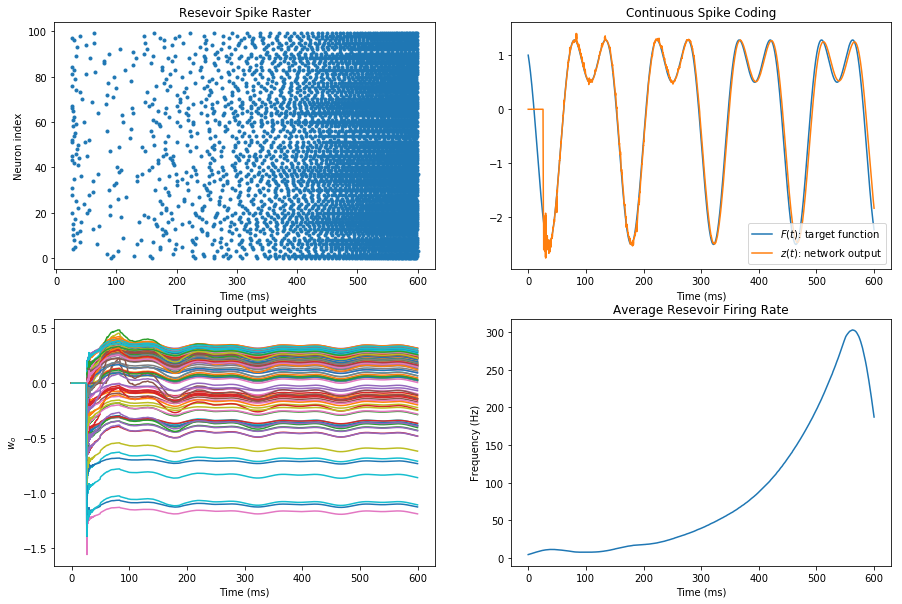
\includegraphics{N100.png}
\caption{N = 100}
\end{figure}

\begin{center}\rule{0.5\linewidth}{\linethickness}\end{center}

Let's look more closely at the target function and network output:

    \begin{Verbatim}[commandchars=\\\{\}]
{\color{incolor}In [{\color{incolor}8}]:} \PY{n}{figure}\PY{p}{(}\PY{n}{figsize}\PY{o}{=}\PY{p}{[}\PY{l+m+mi}{10}\PY{p}{,}\PY{l+m+mi}{6}\PY{p}{]}\PY{p}{)}
        
        \PY{n}{plot}\PY{p}{(}\PY{n}{inMon}\PY{o}{.}\PY{n}{t}\PY{o}{/}\PY{n}{ms}\PY{p}{,} \PY{n}{inMon}\PY{o}{.}\PY{n}{F}\PY{o}{.}\PY{n}{flatten}\PY{p}{(}\PY{p}{)}\PY{p}{,}\PY{n}{ls}\PY{o}{=}\PY{l+s+s1}{\PYZsq{}}\PY{l+s+s1}{\PYZhy{}\PYZhy{}}\PY{l+s+s1}{\PYZsq{}}\PY{p}{,}\PY{n}{lw}\PY{o}{=}\PY{l+m+mi}{2}\PY{p}{,}\PY{n}{label}\PY{o}{=}\PY{l+s+s1}{\PYZsq{}}\PY{l+s+s1}{\PYZdl{}F(t)\PYZdl{}: target function}\PY{l+s+s1}{\PYZsq{}}\PY{p}{)}
        \PY{n}{plot}\PY{p}{(}\PY{n}{outMon}\PY{o}{.}\PY{n}{t}\PY{o}{/}\PY{n}{ms}\PY{p}{,} \PY{n}{outMon}\PY{o}{.}\PY{n}{z}\PY{o}{.}\PY{n}{flatten}\PY{p}{(}\PY{p}{)}\PY{p}{,}\PY{n}{lw}\PY{o}{=}\PY{l+m+mi}{2}\PY{p}{,}\PY{n}{label}\PY{o}{=}\PY{l+s+s1}{\PYZsq{}}\PY{l+s+s1}{\PYZdl{}z(t)\PYZdl{}: network output}\PY{l+s+s1}{\PYZsq{}}\PY{p}{)}
        \PY{n}{plot}\PY{p}{(}\PY{n}{outMon}\PY{o}{.}\PY{n}{t}\PY{o}{/}\PY{n}{ms}\PY{p}{,} \PY{n}{outMon}\PY{o}{.}\PY{n}{z}\PY{o}{.}\PY{n}{flatten}\PY{p}{(}\PY{p}{)} \PY{o}{\PYZhy{}} \PY{n}{inMon}\PY{o}{.}\PY{n}{F}\PY{o}{.}\PY{n}{flatten}\PY{p}{(}\PY{p}{)}\PY{p}{,} \PY{n}{label}\PY{o}{=}\PY{l+s+s1}{\PYZsq{}}\PY{l+s+s1}{\PYZdl{}e(t)\PYZdl{}: error}\PY{l+s+s1}{\PYZsq{}}\PY{p}{)}
        \PY{n}{grid}\PY{p}{(}\PY{p}{)}
        \PY{n}{title}\PY{p}{(}\PY{l+s+s1}{\PYZsq{}}\PY{l+s+s1}{Coding of arbitrary continuous signals: N=}\PY{l+s+si}{\PYZob{}\PYZcb{}}\PY{l+s+s1}{\PYZsq{}}\PY{o}{.}\PY{n}{format}\PY{p}{(}\PY{n}{N}\PY{p}{)}\PY{p}{)}
        \PY{n}{xlabel}\PY{p}{(}\PY{l+s+s1}{\PYZsq{}}\PY{l+s+s1}{Time (ms)}\PY{l+s+s1}{\PYZsq{}}\PY{p}{)}
        \PY{n}{legend}\PY{p}{(}\PY{n}{loc}\PY{o}{=}\PY{l+s+s1}{\PYZsq{}}\PY{l+s+s1}{lower right}\PY{l+s+s1}{\PYZsq{}}\PY{p}{)}
        \PY{c+c1}{\PYZsh{}xlim([0,400])}
        \PY{n}{show}\PY{p}{(}\PY{p}{)}
\end{Verbatim}


    \begin{center}
    \adjustimage{max size={0.9\linewidth}{0.9\paperheight}}{output_13_0.png}
    \end{center}
    { \hspace*{\fill} \\}
    
    Notice how the error decreases initially, then begins to increase with a
periodic pattern. This is due to the slight accumulated delay of the
network; as time continues, there is a larger and larger phase shift
between \(z(t)\) and \(F(t)\). If we continue training indefinitely with
this periodic driving function, the phase-shifted error eventually
causes a large attenuation of network output \(z(t)\).

\begin{center}\rule{0.5\linewidth}{\linethickness}\end{center}

\hypertarget{recreating-fig-1b-1d}{%
\subsection{Recreating Fig 1b, 1d}\label{recreating-fig-1b-1d}}

    \begin{Verbatim}[commandchars=\\\{\}]
{\color{incolor}In [{\color{incolor}9}]:} \PY{n}{figure}\PY{p}{(}\PY{n}{figsize}\PY{o}{=}\PY{p}{[}\PY{l+m+mi}{10}\PY{p}{,}\PY{l+m+mi}{10}\PY{p}{]}\PY{p}{)}
        \PY{n}{subplot}\PY{p}{(}\PY{l+m+mi}{3}\PY{p}{,}\PY{l+m+mi}{1}\PY{p}{,}\PY{l+m+mi}{1}\PY{p}{)}
        \PY{k}{for} \PY{n}{i} \PY{o+ow}{in} \PY{n+nb}{range}\PY{p}{(}\PY{l+m+mi}{10}\PY{p}{)}\PY{p}{:}
            \PY{n}{plot}\PY{p}{(}\PY{n}{resMon}\PY{o}{.}\PY{n}{t}\PY{o}{/}\PY{n}{ms}\PY{p}{,} \PY{n}{resMon}\PY{o}{.}\PY{n}{V}\PY{p}{[}\PY{n}{i}\PY{p}{]}\PY{o}{+}\PY{l+m+mf}{0.2}\PY{o}{*}\PY{n}{i}\PY{p}{)}
        \PY{n}{xlabel}\PY{p}{(}\PY{l+s+s1}{\PYZsq{}}\PY{l+s+s1}{\PYZsq{}}\PY{p}{)}
        \PY{n}{tick\PYZus{}params}\PY{p}{(}\PY{n}{bottom}\PY{o}{=}\PY{k+kc}{False}\PY{p}{,} \PY{n}{labelbottom}\PY{o}{=}\PY{k+kc}{False}\PY{p}{,} \PY{n}{labelleft}\PY{o}{=}\PY{k+kc}{False}\PY{p}{)}\PY{c+c1}{\PYZsh{}xlim([0,600])}
        
        \PY{n}{subplot}\PY{p}{(}\PY{l+m+mi}{3}\PY{p}{,}\PY{l+m+mi}{1}\PY{p}{,}\PY{l+m+mi}{2}\PY{p}{)}
        \PY{n}{plot}\PY{p}{(}\PY{n}{inMon}\PY{o}{.}\PY{n}{t}\PY{o}{/}\PY{n}{ms}\PY{p}{,} \PY{n}{inMon}\PY{o}{.}\PY{n}{F}\PY{o}{.}\PY{n}{flatten}\PY{p}{(}\PY{p}{)}\PY{p}{,}\PY{n}{ls}\PY{o}{=}\PY{l+s+s1}{\PYZsq{}}\PY{l+s+s1}{\PYZhy{}\PYZhy{}}\PY{l+s+s1}{\PYZsq{}}\PY{p}{,}\PY{n}{lw}\PY{o}{=}\PY{l+m+mi}{2}\PY{p}{,}\PY{n}{label}\PY{o}{=}\PY{l+s+s1}{\PYZsq{}}\PY{l+s+s1}{\PYZdl{}F(t)\PYZdl{}: target function}\PY{l+s+s1}{\PYZsq{}}\PY{p}{)}
        \PY{n}{plot}\PY{p}{(}\PY{n}{outMon}\PY{o}{.}\PY{n}{t}\PY{o}{/}\PY{n}{ms}\PY{p}{,} \PY{n}{outMon}\PY{o}{.}\PY{n}{z}\PY{o}{.}\PY{n}{flatten}\PY{p}{(}\PY{p}{)}\PY{p}{,}\PY{n}{lw}\PY{o}{=}\PY{l+m+mi}{2}\PY{p}{,}\PY{n}{label}\PY{o}{=}\PY{l+s+s1}{\PYZsq{}}\PY{l+s+s1}{\PYZdl{}z(t)\PYZdl{}: network output}\PY{l+s+s1}{\PYZsq{}}\PY{p}{)}
        \PY{n}{tick\PYZus{}params}\PY{p}{(}\PY{n}{bottom}\PY{o}{=}\PY{k+kc}{False}\PY{p}{,} \PY{n}{labelbottom}\PY{o}{=}\PY{k+kc}{False}\PY{p}{)}
        \PY{n}{legend}\PY{p}{(}\PY{n}{loc}\PY{o}{=}\PY{l+s+s1}{\PYZsq{}}\PY{l+s+s1}{lower right}\PY{l+s+s1}{\PYZsq{}}\PY{p}{)}
        \PY{n}{grid}\PY{p}{(}\PY{p}{)}
        
        \PY{n}{subplot}\PY{p}{(}\PY{l+m+mi}{3}\PY{p}{,}\PY{l+m+mi}{1}\PY{p}{,}\PY{l+m+mi}{3}\PY{p}{)}
        \PY{n}{plot}\PY{p}{(}\PY{n}{resSpikeMon}\PY{o}{.}\PY{n}{t}\PY{o}{/}\PY{n}{ms}\PY{p}{,} \PY{n}{resSpikeMon}\PY{o}{.}\PY{n}{i}\PY{p}{,}\PY{l+s+s1}{\PYZsq{}}\PY{l+s+s1}{.}\PY{l+s+s1}{\PYZsq{}}\PY{p}{,} \PY{n}{label}\PY{o}{=}\PY{l+s+s1}{\PYZsq{}}\PY{l+s+s1}{\PYZdl{}s\PYZus{}N(t)\PYZdl{}: spike trains}\PY{l+s+s1}{\PYZsq{}}\PY{p}{)}
        \PY{c+c1}{\PYZsh{}ylabel(\PYZsq{}Spike trains: \PYZdl{}s\PYZus{}N(t)\PYZdl{}\PYZsq{})}
        \PY{n}{xlabel}\PY{p}{(}\PY{l+s+s1}{\PYZsq{}}\PY{l+s+s1}{Time (ms)}\PY{l+s+s1}{\PYZsq{}}\PY{p}{)}
        \PY{n}{legend}\PY{p}{(}\PY{n}{loc}\PY{o}{=}\PY{l+s+s1}{\PYZsq{}}\PY{l+s+s1}{lower right}\PY{l+s+s1}{\PYZsq{}}\PY{p}{)}
        \PY{n}{show}\PY{p}{(}\PY{p}{)}
\end{Verbatim}


    \begin{center}
    \adjustimage{max size={0.9\linewidth}{0.9\paperheight}}{output_15_0.png}
    \end{center}
    { \hspace*{\fill} \\}
    
    \begin{center}\rule{0.5\linewidth}{\linethickness}\end{center}

\hypertarget{self-sustained-activity}{%
\subsubsection{Self-sustained activity?}\label{self-sustained-activity}}

The true hallmark of spike-based universal computation is self-sustained
activity, without any driving function input. Now that we've trained the
network, we can attempt to elicit continued periodic output.

Unfortunately, one drawback of the paper is a lack of clear input to the
system. In the case of modeling a weighted pendulum, they describe an
exploratory white noise input. Otherwise, no clear decription for model
input during the testing phase is given. I have attempted here to input
Gaussian random noise to elicit a response; as you can see below,
however, this is not successful.

    \begin{Verbatim}[commandchars=\\\{\}]
{\color{incolor}In [{\color{incolor}10}]:} \PY{n}{store}\PY{p}{(}\PY{l+s+s1}{\PYZsq{}}\PY{l+s+s1}{after\PYZus{}training}\PY{l+s+s1}{\PYZsq{}}\PY{p}{)}
\end{Verbatim}


    \begin{Verbatim}[commandchars=\\\{\}]
{\color{incolor}In [{\color{incolor}11}]:} \PY{c+c1}{\PYZsh{}\PYZsh{}\PYZsh{}\PYZsh{}\PYZsh{}\PYZsh{}\PYZsh{}\PYZsh{}\PYZsh{}\PYZsh{}\PYZsh{}\PYZsh{}\PYZsh{}\PYZsh{}\PYZsh{}\PYZsh{}\PYZsh{}\PYZsh{}\PYZsh{}\PYZsh{}\PYZsh{}\PYZsh{}\PYZsh{}\PYZsh{}\PYZsh{}\PYZsh{}\PYZsh{}\PYZsh{}\PYZsh{}\PYZsh{}\PYZsh{}\PYZsh{}\PYZsh{}\PYZsh{}\PYZsh{}\PYZsh{}\PYZsh{}\PYZsh{}\PYZsh{}\PYZsh{}\PYZsh{}\PYZsh{}\PYZsh{}\PYZsh{}\PYZsh{}\PYZsh{}\PYZsh{}\PYZsh{}\PYZsh{}\PYZsh{}\PYZsh{}\PYZsh{}\PYZsh{}\PYZsh{}\PYZsh{}\PYZsh{}\PYZsh{}\PYZsh{}\PYZsh{}\PYZsh{}\PYZsh{}\PYZsh{}\PYZsh{}\PYZsh{}\PYZsh{}\PYZsh{}\PYZsh{}\PYZsh{}\PYZsh{}\PYZsh{}\PYZsh{}\PYZsh{}\PYZsh{}\PYZsh{}\PYZsh{}\PYZsh{}\PYZsh{}\PYZsh{}\PYZsh{}\PYZsh{}}
         \PY{c+c1}{\PYZsh{} Testing phase}
         \PY{c+c1}{\PYZsh{}\PYZsh{}\PYZsh{}\PYZsh{}\PYZsh{}\PYZsh{}\PYZsh{}\PYZsh{}\PYZsh{}\PYZsh{}\PYZsh{}\PYZsh{}\PYZsh{}\PYZsh{}\PYZsh{}\PYZsh{}\PYZsh{}\PYZsh{}\PYZsh{}\PYZsh{}\PYZsh{}\PYZsh{}\PYZsh{}\PYZsh{}\PYZsh{}\PYZsh{}\PYZsh{}\PYZsh{}\PYZsh{}\PYZsh{}\PYZsh{}\PYZsh{}\PYZsh{}\PYZsh{}\PYZsh{}\PYZsh{}\PYZsh{}\PYZsh{}\PYZsh{}\PYZsh{}\PYZsh{}\PYZsh{}\PYZsh{}\PYZsh{}\PYZsh{}\PYZsh{}\PYZsh{}\PYZsh{}\PYZsh{}\PYZsh{}\PYZsh{}\PYZsh{}\PYZsh{}\PYZsh{}\PYZsh{}\PYZsh{}\PYZsh{}\PYZsh{}\PYZsh{}\PYZsh{}\PYZsh{}\PYZsh{}\PYZsh{}\PYZsh{}\PYZsh{}\PYZsh{}\PYZsh{}\PYZsh{}\PYZsh{}\PYZsh{}\PYZsh{}\PYZsh{}\PYZsh{}\PYZsh{}\PYZsh{}\PYZsh{}\PYZsh{}\PYZsh{}\PYZsh{}\PYZsh{}}
         
         \PY{n}{restore}\PY{p}{(}\PY{l+s+s1}{\PYZsq{}}\PY{l+s+s1}{after\PYZus{}training}\PY{l+s+s1}{\PYZsq{}}\PY{p}{)}
         
         \PY{c+c1}{\PYZsh{} Turn off synaptic plasticity in output weights}
         \PY{n}{outsyn}\PY{o}{.}\PY{n}{plastic} \PY{o}{=} \PY{k+kc}{False}
         
         \PY{c+c1}{\PYZsh{} Switch input neuron from signal to Gaussian noise with amplitude `noiseAmp`}
         \PY{n}{inneur}\PY{o}{.}\PY{n}{training} \PY{o}{=} \PY{k+kc}{False}
         \PY{n}{inneur}\PY{o}{.}\PY{n}{noiseAmp} \PY{o}{=} \PY{l+m+mf}{0.1}
\end{Verbatim}


    \begin{Verbatim}[commandchars=\\\{\}]
{\color{incolor}In [{\color{incolor}12}]:} \PY{c+c1}{\PYZsh{} Run for 100 ms}
         \PY{n}{testDur} \PY{o}{=} \PY{l+m+mi}{200}\PY{o}{*}\PY{n}{ms}
         \PY{n}{run}\PY{p}{(}\PY{n}{testDur}\PY{p}{)}
\end{Verbatim}


    \begin{Verbatim}[commandchars=\\\{\}]
{\color{incolor}In [{\color{incolor}13}]:} \PY{c+c1}{\PYZsh{} Plot feedback current}
         \PY{n}{figure}\PY{p}{(}\PY{n}{figsize}\PY{o}{=}\PY{p}{[}\PY{l+m+mi}{14}\PY{p}{,}\PY{l+m+mi}{6}\PY{p}{]}\PY{p}{)}
         \PY{n}{subplot}\PY{p}{(}\PY{l+m+mi}{121}\PY{p}{)}
         \PY{k}{for} \PY{n}{i} \PY{o+ow}{in} \PY{n+nb}{range}\PY{p}{(}\PY{n}{N}\PY{p}{)}\PY{p}{:}
             \PY{n}{plot}\PY{p}{(}\PY{n}{resMon}\PY{o}{.}\PY{n}{t}\PY{o}{/}\PY{n}{ms}\PY{p}{,} \PY{n}{resMon}\PY{o}{.}\PY{n}{Ifb}\PY{p}{[}\PY{n}{i}\PY{p}{]}\PY{p}{)}
         \PY{n}{axvline}\PY{p}{(}\PY{p}{(}\PY{n}{resMon}\PY{o}{.}\PY{n}{t}\PY{p}{[}\PY{o}{\PYZhy{}}\PY{l+m+mi}{1}\PY{p}{]} \PY{o}{\PYZhy{}} \PY{n}{testDur}\PY{p}{)}\PY{o}{/}\PY{n}{ms}\PY{p}{,} \PY{n}{ls}\PY{o}{=}\PY{l+s+s1}{\PYZsq{}}\PY{l+s+s1}{\PYZhy{}\PYZhy{}}\PY{l+s+s1}{\PYZsq{}}\PY{p}{,}\PY{n}{c}\PY{o}{=}\PY{l+s+s1}{\PYZsq{}}\PY{l+s+s1}{C3}\PY{l+s+s1}{\PYZsq{}}\PY{p}{)}
         \PY{n}{xlabel}\PY{p}{(}\PY{l+s+s1}{\PYZsq{}}\PY{l+s+s1}{Time (ms)}\PY{l+s+s1}{\PYZsq{}}\PY{p}{)}
         \PY{n}{ylabel}\PY{p}{(}\PY{l+s+s1}{\PYZsq{}}\PY{l+s+s1}{Current}\PY{l+s+s1}{\PYZsq{}}\PY{p}{)}
         \PY{n}{title}\PY{p}{(}\PY{l+s+s1}{\PYZsq{}}\PY{l+s+s1}{\PYZdl{}I\PYZus{}}\PY{l+s+si}{\PYZob{}fb\PYZcb{}}\PY{l+s+s1}{\PYZdl{} over training and testing}\PY{l+s+s1}{\PYZsq{}}\PY{p}{)}
         
         \PY{n}{subplot}\PY{p}{(}\PY{l+m+mi}{122}\PY{p}{)}
         \PY{n}{plot}\PY{p}{(}\PY{n}{resSpikeMon}\PY{o}{.}\PY{n}{t}\PY{o}{/}\PY{n}{ms}\PY{p}{,} \PY{n}{resSpikeMon}\PY{o}{.}\PY{n}{i}\PY{p}{,}\PY{l+s+s1}{\PYZsq{}}\PY{l+s+s1}{.}\PY{l+s+s1}{\PYZsq{}}\PY{p}{)}
         \PY{n}{axvline}\PY{p}{(}\PY{p}{(}\PY{n}{resMon}\PY{o}{.}\PY{n}{t}\PY{p}{[}\PY{o}{\PYZhy{}}\PY{l+m+mi}{1}\PY{p}{]} \PY{o}{\PYZhy{}} \PY{n}{testDur}\PY{p}{)}\PY{o}{/}\PY{n}{ms}\PY{p}{,} \PY{n}{ls}\PY{o}{=}\PY{l+s+s1}{\PYZsq{}}\PY{l+s+s1}{\PYZhy{}\PYZhy{}}\PY{l+s+s1}{\PYZsq{}}\PY{p}{,}\PY{n}{c}\PY{o}{=}\PY{l+s+s1}{\PYZsq{}}\PY{l+s+s1}{C3}\PY{l+s+s1}{\PYZsq{}}\PY{p}{)}
         \PY{n}{title}\PY{p}{(}\PY{l+s+s1}{\PYZsq{}}\PY{l+s+s1}{Resevoir Spike Raster}\PY{l+s+s1}{\PYZsq{}}\PY{p}{)}
         \PY{n}{xlabel}\PY{p}{(}\PY{l+s+s1}{\PYZsq{}}\PY{l+s+s1}{Time (ms)}\PY{l+s+s1}{\PYZsq{}}\PY{p}{)}
         \PY{n}{ylabel}\PY{p}{(}\PY{l+s+s1}{\PYZsq{}}\PY{l+s+s1}{Neuron index}\PY{l+s+s1}{\PYZsq{}}\PY{p}{)}
         \PY{n}{show}\PY{p}{(}\PY{p}{)}
\end{Verbatim}


    \begin{center}
    \adjustimage{max size={0.9\linewidth}{0.9\paperheight}}{output_20_0.png}
    \end{center}
    { \hspace*{\fill} \\}
    
    To view our output, let's now plot the feedback currents: note the
periodic signal (based on network output) before the testing phase
begins (vertical red dashed line), versus the random growing noise
during the testing phase. We also see a rapid increase in spike rate,
despite not truly encoding our signal.

Finally, our (unsuccessful) output function:

    \begin{Verbatim}[commandchars=\\\{\}]
{\color{incolor}In [{\color{incolor}14}]:} \PY{n}{figure}\PY{p}{(}\PY{n}{figsize}\PY{o}{=}\PY{p}{[}\PY{l+m+mi}{10}\PY{p}{,}\PY{l+m+mi}{6}\PY{p}{]}\PY{p}{)}
         \PY{n}{plot}\PY{p}{(}\PY{n}{outMon}\PY{o}{.}\PY{n}{t}\PY{o}{/}\PY{n}{ms}\PY{p}{,} \PY{n}{cos}\PY{p}{(}\PY{l+m+mi}{28} \PY{o}{*} \PY{n}{pi} \PY{o}{*} \PY{n}{Hz} \PY{o}{*} \PY{n}{outMon}\PY{o}{.}\PY{n}{t}\PY{p}{)} \PY{o}{\PYZhy{}} \PY{l+m+mf}{1.5} \PY{o}{*} \PY{n}{sin}\PY{p}{(}\PY{l+m+mi}{14} \PY{o}{*} \PY{n}{pi} \PY{o}{*} \PY{n}{Hz} \PY{o}{*} \PY{n}{outMon}\PY{o}{.}\PY{n}{t}\PY{p}{)}\PY{p}{,}\PY{n}{ls}\PY{o}{=}\PY{l+s+s1}{\PYZsq{}}\PY{l+s+s1}{\PYZhy{}\PYZhy{}}\PY{l+s+s1}{\PYZsq{}}\PY{p}{,}\PY{n}{lw}\PY{o}{=}\PY{l+m+mi}{2}\PY{p}{,}\PY{n}{label}\PY{o}{=}\PY{l+s+s1}{\PYZsq{}}\PY{l+s+s1}{\PYZdl{}F(t)\PYZdl{}: target function}\PY{l+s+s1}{\PYZsq{}}\PY{p}{)}
         \PY{n}{plot}\PY{p}{(}\PY{n}{outMon}\PY{o}{.}\PY{n}{t}\PY{o}{/}\PY{n}{ms}\PY{p}{,} \PY{n}{outMon}\PY{o}{.}\PY{n}{z}\PY{o}{.}\PY{n}{flatten}\PY{p}{(}\PY{p}{)}\PY{p}{,}\PY{n}{lw}\PY{o}{=}\PY{l+m+mi}{2}\PY{p}{,}\PY{n}{label}\PY{o}{=}\PY{l+s+s1}{\PYZsq{}}\PY{l+s+s1}{\PYZdl{}z(t)\PYZdl{}: network output}\PY{l+s+s1}{\PYZsq{}}\PY{p}{)}
         \PY{n}{axvline}\PY{p}{(}\PY{p}{(}\PY{n}{resMon}\PY{o}{.}\PY{n}{t}\PY{p}{[}\PY{o}{\PYZhy{}}\PY{l+m+mi}{1}\PY{p}{]} \PY{o}{\PYZhy{}} \PY{n}{testDur}\PY{p}{)}\PY{o}{/}\PY{n}{ms}\PY{p}{,} \PY{n}{ls}\PY{o}{=}\PY{l+s+s1}{\PYZsq{}}\PY{l+s+s1}{\PYZhy{}\PYZhy{}}\PY{l+s+s1}{\PYZsq{}}\PY{p}{,}\PY{n}{c}\PY{o}{=}\PY{l+s+s1}{\PYZsq{}}\PY{l+s+s1}{C3}\PY{l+s+s1}{\PYZsq{}}\PY{p}{)}
         \PY{n}{legend}\PY{p}{(}\PY{n}{loc}\PY{o}{=}\PY{l+s+s1}{\PYZsq{}}\PY{l+s+s1}{upper left}\PY{l+s+s1}{\PYZsq{}}\PY{p}{)}
         \PY{n}{title}\PY{p}{(}\PY{l+s+s1}{\PYZsq{}}\PY{l+s+s1}{Continuous Spike Code: Testing Sustained Activity}\PY{l+s+s1}{\PYZsq{}}\PY{p}{)}
         \PY{n}{xlabel}\PY{p}{(}\PY{l+s+s1}{\PYZsq{}}\PY{l+s+s1}{Time (ms)}\PY{l+s+s1}{\PYZsq{}}\PY{p}{)}
         \PY{n}{grid}\PY{p}{(}\PY{p}{)}
         \PY{n}{show}\PY{p}{(}\PY{p}{)}
\end{Verbatim}


    \begin{center}
    \adjustimage{max size={0.9\linewidth}{0.9\paperheight}}{output_22_0.png}
    \end{center}
    { \hspace*{\fill} \\}
    
    \begin{center}\rule{0.5\linewidth}{\linethickness}\end{center}

\hypertarget{conclusions}{%
\subsection{Conclusions}\label{conclusions}}

    The universal spike-based computation described in Thalmeier \emph{et
al.}, 2016 is quite interesting. In particular, it seems to be amenable
to a wider range of neuron models than similar models (like the Machens
\& Deneve, 2016 model I implemented in my qualifying exam). However, I
believe that the Deneve approach is more elegant than this spike coding
approach. Here, though the authors describe this system as ``spike
coding,'' the timing relation between individual spikes is not enforced.
In other words, the authors do not enforce the tight temporal coupling
between excitation and inhibition that marks the Deneve computation
approach. As such, sparsity is not controlled as directly in the
approach demonstrated here.

That said, this training method is far more efficient than the post-hoc
\(l_2\)-minimization described in Abbott \emph{et al}, 2016. In fact,
on-line FORCE learning and recursive least squares optimization could
perhaps be usefully implemented in those rate-based coding methods.

I write ``spike coding'' here in scare quotes because information is not
direcly encoded in order of spikes, or in time interval between spikes
of different neurons, but in summed post-synaptic fluctuations of the
neurons \(r(t)\). In my opinion, this is much closer to the rate-coded
networks described in Abbott \emph{et al.}, 2016 (or DePasquale,
Churchland, and Abbott 2016) than Deneve's spike coding network. Even
after implementing these spike coding network, I am still partial to
Deneve's tightly-balanced networks.


    % Add a bibliography block to the postdoc
    
    
    
    \end{document}
